% ══════════════════════════════════════════════════════════════════════════════
%  DATect Paper --- MDPI Toxins Format
%  Converted from elsarticle format with expanded content
% ══════════════════════════════════════════════════════════════════════════════

\PassOptionsToPackage{xetex}{xcolor}
\documentclass[toxins,article,submit,moreauthors]{Definitions/mdpi}

% ── Additional Packages ─────────────────────────────────────────────────────
\usepackage{amsmath,amssymb}
\usepackage{siunitx}
\usepackage{tabularx}
\usepackage{multirow}
\usepackage[ruled,vlined]{algorithm2e}
\usepackage{enumitem}

% ── SI units ─────────────────────────────────────────────────────────────────
\DeclareSIUnit{\microgrampeg}{\ensuremath{\mu}g/g}
\DeclareSIUnit{\cellsperL}{cells/L}

% ── MDPI internal commands ───────────────────────────────────────────────────
\firstpage{1}
\makeatletter
\setcounter{page}{\@firstpage}
\makeatother
\pubvolume{1}
\issuenum{1}
\articlenumber{0}
\pubyear{2026}
\copyrightyear{2026}
\datereceived{ }
\daterevised{ }
\dateaccepted{ }
\datepublished{ }
\hreflink{https://doi.org/}

% ══════════════════════════════════════════════════════════════════════════════
%  METADATA
% ══════════════════════════════════════════════════════════════════════════════

\Title{DATect: Per-Site Machine Learning Forecasting of Domoic Acid Along the Pacific Northwest Coast}

\TitleCitation{DATect: Per-Site ML Forecasting of Domoic Acid in the Pacific Northwest}

\newcommand{\orcidauthorA}{0000-0000-0000-000X}

\Author{Anson Chen $^{1,*}$\orcidA{} and John Mickett $^{2}$}

\AuthorNames{Anson Chen and John Mickett}

\AuthorCitation{Chen, A.; Mickett, J.}

\address{%
$^{1}$ \quad Paul G. Allen School of Computer Science \& Engineering, University of Washington, Seattle, WA 98195, USA; ac283@uw.edu\\
$^{2}$ \quad Applied Physics Laboratory, University of Washington, Seattle, WA 98105, USA; mickett@uw.edu}

\corres{Correspondence: ac283@uw.edu}

% ══════════════════════════════════════════════════════════════════════════════
%  ABSTRACT
% ══════════════════════════════════════════════════════════════════════════════
\abstract{
Domoic acid (DA) contamination of shellfish is a recurring public health crisis along the U.S.\ Pacific Northwest coast, yet no quantitative forecasting system has been published for the region. We present DATect, a one-week-ahead site-specific DA forecasting system for 10 monitoring sites spanning \SI{600}{\kilo\meter} of Washington and Oregon coast, trained on 21 years (2003--2023) of satellite, climate, hydrological, and biological data. DATect couples a per-site XGBoost + Random Forest ensemble with a transition-focused binary classifier; all per-site configuration is selected by leak-free chronological cross-validation on pre-2022 data, making the 2022--2023 temporal holdout fully unbiased. On that holdout (every real DA measurement, $N = 409$), the regression ensemble achieves pooled $R^2 = 0.419$ [95\% CI: 0.247, 0.546], MAE $= \SI{7.49}{\microgrampeg}$, and spike recall $= 0.774$ for the \SI{20}{\microgrampeg} regulatory threshold (alerting at a forecast of \SI{12}{\microgrampeg}), with positive skill at 8 of the 9 sites that have holdout measurements. Combining the regression with the transition classifier detects 92.1\% of spikes and 76.3\% of new spike onsets on a 2,105-point retrospective sample, versus 11.8\% of onsets for na\"ive persistence. DATect is deployed as a publicly accessible web dashboard.
}

\keyword{domoic acid; harmful algal blooms; machine learning; ensemble forecasting; \textit{Pseudo-nitzschia}; Pacific Northwest; XGBoost; data leakage prevention}

% ══════════════════════════════════════════════════════════════════════════════
%  DOCUMENT
% ══════════════════════════════════════════════════════════════════════════════
\begin{document}

% ══════════════════════════════════════════════════════════════════════════════
%  1. INTRODUCTION
% ══════════════════════════════════════════════════════════════════════════════
\section{Introduction}
\label{sec:introduction}

% ── 1.1 DA Biology, Drivers, and Impacts ─────────────────────────────────────
\subsection{Domoic Acid and \textit{Pseudo-nitzschia} Blooms}
\label{sec:intro-biology}

Domoic acid (DA) is a potent neurotoxin produced by certain species of the marine diatom genus \textit{Pseudo-nitzschia} and is the causative agent of amnesic shellfish poisoning \cite{Bates2018, Trainer2012, Wright1989}. Since the first documented global outbreak in 1987, DA contamination has become a persistent threat along the U.S.\ Pacific coast, with severe consequences for human health, coastal economies, and marine wildlife \cite{Mos2001, Lefebvre2010, Trainer2012}. The 2015 marine heatwave illustrates the scale of this risk: DA concentrations in razor clams exceeded the federal safety limit by over 700\%, causing tens of millions of dollars in fishery losses \cite{McCabe2016, Bond2015, Trainer2020}.

Forecasting DA is difficult because toxin production is only weakly coupled to bloom magnitude. DA production depends strongly on physiological stress---particularly nutrient limitation---so a large \textit{Pseudo-nitzschia} bloom may be weakly toxic while a smaller bloom generates dangerous contamination \cite{Trick2010, Marchetti2004, Lelong2012}. In the Pacific Northwest (PNW), this biology interacts with coastal upwelling, climate variability, and retention zones such as the Juan de Fuca eddy and Heceta Bank, creating a multiscale nonlinear system with strong spatial heterogeneity \cite{Trainer2002, Trainer2009, McKibben2017, Jacox2018}.

% ── 1.2 Existing Monitoring and Forecasting ──────────────────────────────────
\subsection{Existing Monitoring and Forecasting in the Pacific Northwest}
\label{sec:intro-monitoring}

Current DA risk management in the PNW is reactive: beaches are closed only after measured toxin levels exceed the FDA regulatory limit of \SI{20}{\microgrampeg} \cite{McCabe2023}, giving managers no advance warning. The primary forecasting tool is the NOAA Pacific Northwest HAB Bulletin \cite{McCabe2023}, issued biweekly to monthly during peak bloom season. The Bulletin synthesizes environmental and biological data into qualitative risk categories (low/medium/high) that provide strategic planning value \cite{Jin2024} but do not produce numerical DA predictions and operate at seasonal rather than weekly resolution. Complementary regional resources include Oregon's phytoplankton monitoring program \cite{McKibben2015} and the SoundToxins network \cite{Trainer2023}, which extend field observations of harmful phytoplankton and toxins, together with the LiveOcean circulation model \cite{MacCready2021}, which supplies numerically simulated coastal and estuarine circulation fields; none of these systems produce numerical DA forecasts. The California C-HARM system \cite{Anderson2016} provides bloom-probability nowcasts for California but does not extend to Washington or Oregon (Table~\ref{tab:system-comparison}).

A critical gap thus exists: \textbf{no quantitative DA concentration forecasting system has been developed for the Pacific Northwest}. All existing monitoring is reactive, and the sole forecasting tool provides qualitative risk categories, not numerical toxin predictions.

% ── 1.3 Problem Statement ────────────────────────────────────────────────────
\subsection{Problem Statement and Contributions}
\label{sec:intro-problem}

This paper addresses the absence of quantitative DA forecasting in the PNW by developing DATect, the first system to produce site-specific, numerical DA concentration predictions for this region. We formalize the prediction task as follows: given environmental features available at time $t - 7$ days (the ``anchor date''), predict the DA concentration (\si{\microgrampeg}) at time $t$ for a specific monitoring site $s$ among 10 Pacific Coast locations.

Two evaluation targets matter operationally. The first is magnitude forecasting: how accurately can a system predict DA concentration one week ahead? The second is transition detection: can the system anticipate below-to-above-threshold crossings at \SI{20}{\microgrampeg}, the events that trigger harvest closures? DATect is evaluated on both targets because a model can achieve low average regression error while still missing the closure-relevant transitions that matter most to managers.

This task presents four compounding challenges:
\begin{enumerate}[nosep]
    \item \textbf{Sparse, irregular target variable}: DA measurements are collected approximately weekly but with frequent gaps, missingness, and inconsistent timing across sites.
    \item \textbf{High spatial variability}: The 10 monitoring sites span 5\textdegree\ of latitude ($\sim$\SI{600}{\kilo\meter}), with dramatically different oceanographic regimes, bloom histories, and DA dynamics.
    \item \textbf{Extreme value distribution}: DA measurements are dominated by zeros and low values, with rare but consequential spikes exceeding \SI{100}{\microgrampeg}.
    \item \textbf{Strict temporal integrity requirements}: Operational forecasting demands that no future information leak into predictions, requiring rigorous validation protocols.
\end{enumerate}

This paper makes five main contributions:
\begin{enumerate}[nosep]
    \item \textbf{Quantitative PNW DA forecasting under a strict 3-window chronological protocol}: DATect provides the first site-specific, one-week-ahead DA concentration forecasts for Washington and Oregon, using 21 years of data across 10 monitoring sites. All configuration decisions (per-site ensemble weights, prediction clipping) are selected via leak-free chronological cross-validation on pre-2022 data only, making the 2022--2023 temporal holdout a fully unbiased generalization estimate.
    \item \textbf{Per-site modeling on sparse, irregular records}: Per-site XGBoost or Random Forest configurations, interpolated training, and raw-only persistence features provide a practical approach to sparse monitoring data while keeping evaluation tied to real observations.
    \item \textbf{Transition-focused early warning}: A dedicated binary spike classifier, pooled across all sites and refit at every forecast, provides advance warning for below-to-above-threshold crossings that trigger harvest closures, complementing the regression forecast rather than replacing it (Section~\ref{sec:results-spike}).
    \item \textbf{Evidence that data quality is the binding constraint}: The Washington--Oregon performance split shows that monitoring density and regularity, not model complexity, are the primary limits on forecast skill in the current regional record.
    \item \textbf{Fully reproducible tuning workflow}: All tunable hyperparameters and chronological evaluation windows are stored in a single source-of-truth JSON file (\texttt{config/tuned\_hyperparameters.json}) with per-key provenance, enabling reviewers and future contributors to re-run the entire selection workflow and reproduce the headline numbers end-to-end.
\end{enumerate}


% ══════════════════════════════════════════════════════════════════════════════
%  2. RELATED WORK
% ══════════════════════════════════════════════════════════════════════════════
\section{Related Work}
\label{sec:related-work}

\subsection{Quantitative Forecasting of Domoic Acid and \textit{Pseudo-nitzschia}}
\label{sec:rw-da-forecasting}

Despite decades of DA monitoring and multiple qualitative forecasting systems, quantitative computational approaches specifically targeting DA or \textit{Pseudo-nitzschia} remain limited in number, geographic scope, and temporal extent \cite{Anderson2012, McGillicuddy2010}.

In the Galician R\'ias Baixas region of northwest Spain, Al\'aez et al.\ \cite{Alaez2021} applied Random Forest and AdaBoost classifiers to predict \textit{Pseudo-nitzschia} bloom events, achieving approximately 85\% classification accuracy. Their study covered five monitoring stations over approximately a decade of data, targeting bloom occurrence (binary classification) rather than DA concentration. Cusack et al.\ \cite{Cusack2015} modeled \textit{Pseudo-nitzschia} events off southwest Ireland using environmental predictors, demonstrating the potential of empirical models for bloom forecasting in European waters. Additional studies have documented \textit{Pseudo-nitzschia} dynamics and DA contamination in new regions, including the Gulf of Maine \cite{Clark2021} and southern Florida \cite{Schreiber2023}, reflecting the global expansion of DA monitoring efforts.

In the California Current, Lane et al.\ \cite{Lane2009} developed a logistic regression model for predicting toxigenic \textit{Pseudo-nitzschia} blooms in Monterey Bay using 8.3 years of monitoring data, achieving $\geq$75\% predictive accuracy with chlorophyll~$a$ and silicic acid as primary predictors.

The closest methodological parallel to DATect is the deep learning system developed by Grasso et al.\ \cite{Grasso2019} for forecasting paralytic shellfish toxin (PST) levels in coastal Maine. Using a convolutional neural network (CNN) trained on chemical data from routine monitoring sites, their system forecasts PST levels on a weekly basis with over 95\% prediction reliability. However, this system targets a different toxin (PST from \textit{Alexandrium catenella}, not DA from \textit{Pseudo-nitzschia}), covers a smaller geographic area (approximately 10 sites along the Maine coast), and uses approximately five years of data.

The California Harmful Algae Risk Mapping (C-HARM) system \cite{Anderson2016} provides satellite-based nowcasts of \textit{Pseudo-nitzschia} bloom probability and DA risk along the California coast. C-HARM integrates satellite imagery with ocean model output to produce gridded risk maps but operates as a nowcast (current conditions) rather than a forecast and does not extend to Washington or Oregon. Moreno et al.\ \cite{Moreno2022} developed a mechanistic process-based model of \textit{Pseudo-nitzschia} and DA production for the California Current, representing a complementary approach to data-driven methods. Most recently, Brunson et al.\ \cite{Brunson2024} demonstrated molecular forecasting of DA using gene expression (dabA and sit1 coexpression) as a one-week-ahead predictor during a bloom in Monterey Bay, representing an emerging genomics-based approach that could eventually complement satellite- and ML-based systems like DATect.

\subsection{Machine Learning Methods for Harmful Algal Blooms}
\label{sec:rw-ml-habs}

Across HAB forecasting more broadly, tree ensembles, linear models, and deep sequence models have all been applied to heterogeneous environmental data \cite{Cruz2021, Shin2024, Hill2020, Yu2021, Manning2019}. For DATect, the most relevant lesson is not that one model family dominates universally, but that coastal forecasting methods must tolerate missingness, nonlinear interactions, and mixed satellite/climate/biological covariates. Gradient boosting and Random Forests therefore provide natural nonlinear competitors \cite{Friedman2001, Chen2016, Breiman2001}, while linear models remain useful baselines for testing whether the gains come from model flexibility or from feature engineering and site-specific design.

\subsection{Data Leakage in Environmental Machine Learning}
\label{sec:rw-leakage}

Recent work has documented the pervasive problem of data leakage in machine learning applications to environmental science. Kapoor and Narayanan \cite{Kapoor2023} demonstrated that data leakage affects a substantial fraction of published ML-based science papers, leading to inflated performance claims and irreproducible results. In temporal prediction tasks such as HAB forecasting, common sources of leakage include random train-test splits that violate temporal ordering, use of features computed from future data, and shared preprocessing across train and test sets \cite{Kaufman2012, Roberts2017, Bergmeir2012}. Proper out-of-sample evaluation for temporal data requires rolling-origin or expanding-window approaches rather than random holdouts \cite{Tashman2000}, and spatial autocorrelation in environmental data further complicates validation design \cite{Valavi2019}.

DATect addresses the leakage problem explicitly through nine structural leakage-prevention mechanisms described in Section~\ref{sec:validation}.

\subsection{Comparison of Existing Systems}
\label{sec:rw-comparison}

Table~\ref{tab:system-comparison} situates DATect among existing systems. To our knowledge, DATect spans the longest temporal record (21 years) and broadest geographic range ($\sim$\SI{600}{\kilo\meter}) of any published quantitative DA or \textit{Pseudo-nitzschia} ML forecasting study.

\begin{table}[H]
\caption{Comparison of existing HAB forecasting systems with DATect.}
\label{tab:system-comparison}
\centering\scriptsize
\begin{tabular*}{\linewidth}{@{\extracolsep{\fill}}lllllll}
\toprule
\textbf{System} & \textbf{Region} & \textbf{Sites} & \textbf{Period} & \textbf{Method} & \textbf{Target} & \textbf{Horizon} \\
\midrule
PNW HAB Bulletin \cite{McCabe2023} & WA/OR & $\sim$20 & 2017-- & Qual.\ expert & DA risk (categ.) & 1--2 wk \\
\addlinespace
Maine PST \cite{Grasso2019} & Maine & $\sim$10 & $\sim$5 yr & CNN & PST (not DA) & 1 wk \\
\addlinespace
Galician RF \cite{Alaez2021} & NW Spain & $\sim$5 & $\sim$10 yr & RF/AdaBoost & PN bloom (bin.) & --- \\
\addlinespace
C-HARM \cite{Anderson2016} & California & Grid & Ongoing & Sat.+model & PN prob. & Nowcast \\
\addlinespace
Monterey Bay LR \cite{Lane2009} & California & 1 & $\sim$8 yr & Logistic reg. & PN bloom (bin.) & --- \\
\addlinespace
\textbf{DATect (this study)} & \textbf{WA/OR} & \textbf{10} & \textbf{21 yr} & \textbf{XGB+RF} & \textbf{DA conc.+categ.} & \textbf{1 wk} \\
\bottomrule
\end{tabular*}
\end{table}


% ══════════════════════════════════════════════════════════════════════════════
%  3. METHODOLOGY
% ══════════════════════════════════════════════════════════════════════════════
\section{Methodology}
\label{sec:methodology}

\subsection{Study Area and Data Collection}
\label{sec:data-collection}

\subsubsection{Monitoring Sites}

DATect forecasts DA concentrations at 10 Pacific Coast monitoring sites spanning from Gold Beach, Oregon (42.38\textdegree\,N) to Kalaloch, Washington (47.59\textdegree\,N), a distance of approximately \SI{600}{\kilo\meter} along the coastline (Figure~\ref{fig:study-area}). Sites were selected for their long historical records, consistent multi-year sampling, and spatial representation across the Washington--Oregon coast. Pacific razor clams (\textit{Siliqua patula}) are sampled at all sites. As filter-feeding bivalves with slow DA depuration (half-life of weeks to months), razor clams continuously accumulate toxin during bloom events, providing an integrated measure of recent DA exposure at each site \cite{Drum1993, Wekell1994, McCabe2023}.

\begin{figure}[H]
\centering
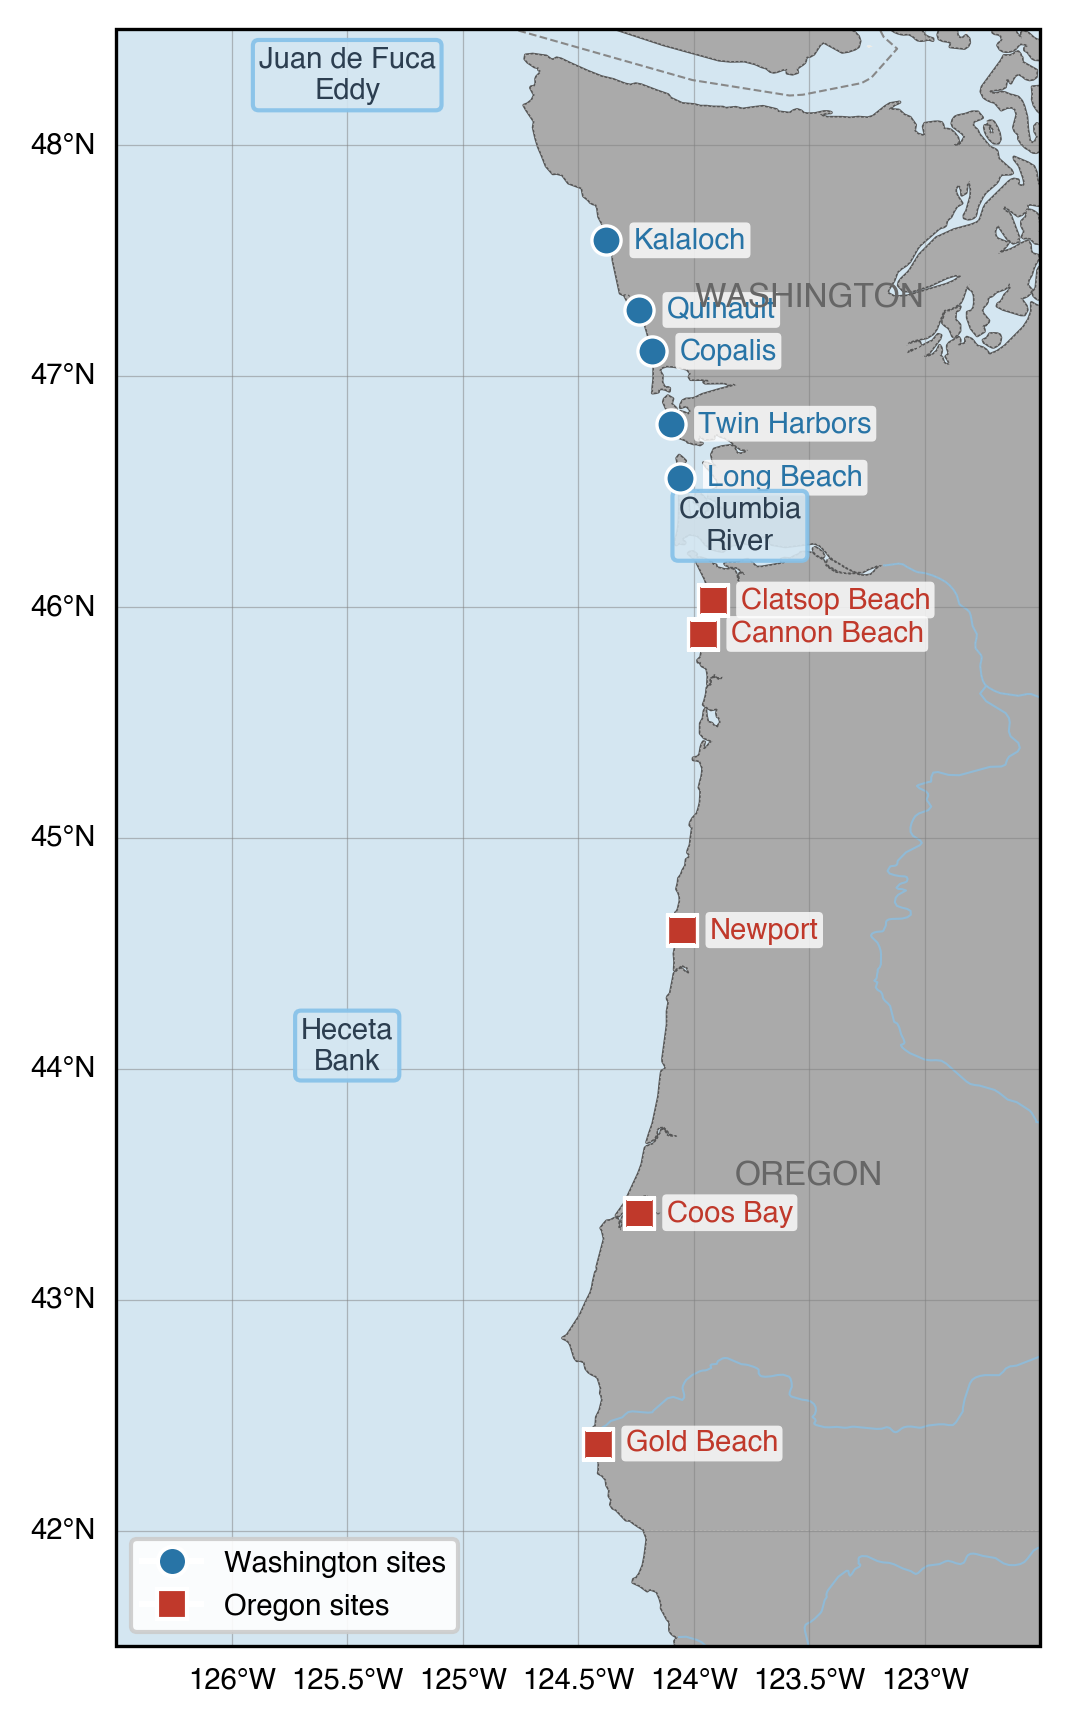
\includegraphics[width=0.55\textwidth]{figures/fig1_study_area.png}
\caption{Study area showing the 10 DATect monitoring sites along the Pacific Northwest coast, spanning $\sim$5\textdegree\ of latitude ($\sim$\SI{600}{\kilo\meter}), with the Juan de Fuca eddy and Heceta Bank retention zones indicated.}
\label{fig:study-area}
\end{figure}

Table~\ref{tab:sites} lists the 10 monitoring sites with their coordinates and the number of validation samples available at each site.

\begin{table}[H]
\caption{DATect monitoring sites, geographic coordinates, and validation sample sizes.}
\label{tab:sites}
\centering\small
\begin{tabular*}{\linewidth}{@{\extracolsep{\fill}}llccc}
\toprule
\textbf{Site} & \textbf{State} & \textbf{Latitude (\textdegree N)} & \textbf{Longitude (\textdegree W)} & \textbf{$N$ (validation)} \\
\midrule
Kalaloch       & WA & 47.586 & 124.379 & 222 \\
Quinault       & WA & 47.284 & 124.236 & 196 \\
Copalis        & WA & 47.106 & 124.181 & 275 \\
Twin Harbors   & WA & 46.792 & 124.100 & 216 \\
Long Beach     & WA & 46.558 & 124.061 & 209 \\
Clatsop Beach  & OR & 46.029 & 123.917 & 309 \\
Cannon Beach   & OR & 45.882 & 123.959 & 118 \\
Newport        & OR & 44.600 & 124.050 & 208 \\
Coos Bay       & OR & 43.376 & 124.237 & 110 \\
Gold Beach     & OR & 42.377 & 124.414 & 242 \\
\midrule
\multicolumn{4}{l}{\textbf{Total validation samples}} & \textbf{2,105} \\
\bottomrule
\end{tabular*}
\end{table}

\subsubsection{Data Sources}

DATect integrates seven categories of environmental and biological data spanning 21 years (2003--2023), summarized in Table~\ref{tab:data-sources}. All data are aligned to a common weekly temporal resolution using Monday-anchored ISO weeks. The dataset is constructed by an automated pipeline that downloads, processes, and integrates all data sources into a unified analysis-ready file.

\begin{table}[H]
\caption{Data sources used in DATect, with temporal resolution, period of record, and operational availability delays enforced during forecasting.}
\label{tab:data-sources}
\centering\footnotesize
\begin{tabularx}{\linewidth}{XXlll}
\toprule
\textbf{Source} & \textbf{Variables} & \textbf{Resolution} & \textbf{Period} & \textbf{Delay} \\
\midrule
MODIS-Aqua (CoastWatch) & Chl-$a$, SST, PAR, FLH, K490 & 8-day, $\sim$\SI{4}{\kilo\meter} & 2003--2023 & 7 d \\
\addlinespace
MODIS anomalies & Chl-$a$ anom., SST anom. & Monthly, $\sim$\SI{4}{\kilo\meter} & 2003--2023 & 2 mo \\
\addlinespace
NOAA ERDDAP & PDO, ONI & Monthly & 2003--2023 & 2 mo \\
\addlinespace
NOAA ERDDAP & BEUTI & Daily & 2003--2023 & 7 d \\
\addlinespace
USGS NWIS & Columbia R.\ discharge & Daily & 2003--2023 & 7 d \\
\addlinespace
WDOH / ODFW & DA concentrations & Irregular ($\sim$wk) & 2003--2023 & --- \\
\addlinespace
WDOH / ODFW & \textit{Pseudo-nitzschia} cells & Irregular & 2003--2023 & --- \\
\bottomrule
\end{tabularx}
\end{table}

Satellite data from MODIS-Aqua \cite{NASA2002} are retrieved as 8-day composites from the NOAA CoastWatch ERDDAP server for each site's local bounding box. The use of 8-day composites mitigates frequent cloud cover in the PNW. A 7-day processing buffer is enforced to simulate operational satellite data availability delays.

Climate indices include the Pacific Decadal Oscillation (PDO) \cite{Mantua1997}, the Oceanic Ni\~no Index (ONI; NOAA operational index based on Ni\~no~3.4 sea surface temperature anomalies in ERSSTv5) \cite{Huang2017}, and the Biologically Effective Upwelling Transport Index (BEUTI) \cite{Jacox2018}. BEUTI is provided at discrete 1\textdegree\ latitude bands; site-specific values are obtained via inverse distance weighting (IDW) to each site's exact latitude. PDO and ONI are subject to a 2-month reporting delay; BEUTI uses a 7-day buffer. Columbia River discharge from the USGS gauge at The Dalles proxies freshwater input to coastal salinity and nutrient dynamics, with the strongest signal at northern Washington sites.

DA measurements and \textit{Pseudo-nitzschia} cell counts were obtained through public records requests to WDOH, WDFW, ODFW, and the Olympic Region Harmful Algal Bloom (ORHAB) Partnership. Measurements reported as below the detection limit ($< 1$~\si{\microgrampeg}) are imputed as $0.5$~\si{\microgrampeg} (half the detection threshold), a standard practice for left-censored environmental data \cite{Helsel2012}. These biological measurements are irregularly spaced, reflecting operational sampling schedules that intensify during suspected bloom events and relax during quiescent periods.

\subsection{Data Engineering}
\label{sec:data-engineering}

\subsubsection{Weekly Aggregation and Gap Handling}

All data are aggregated to Monday-aligned ISO weeks. DA concentrations within each week are aggregated using the \textit{maximum} operation---a conservative choice that preserves worst-case readings for public health relevance. When multiple measurements exist within a single week (common during active bloom monitoring), the maximum ensures that the highest detected toxin level is retained.

Gaps in the DA and \textit{Pseudo-nitzschia} time series are filled using \textit{exponential decay} interpolation. The key reason to prefer this over linear interpolation is temporal integrity: linear interpolation between two measurements requires the \textit{future} measurement to compute intermediate values, introducing data leakage into the gap-filled training targets. Exponential decay propagates information only forward from the last known observation:
\begin{equation}
\hat{y}(t + \Delta t) = y(t) \cdot e^{-\lambda \Delta t}
\label{eq:decay}
\end{equation}
where $y(t)$ is the last observed value, $\Delta t$ is the gap duration in weeks, and $\lambda$ is the species-specific decay rate ($\lambda_{\text{DA}} = 0.2~\text{wk}^{-1}$, half-life $\approx 3.5$ weeks, max gap 2 weeks; $\lambda_{\text{PN}} = 0.3~\text{wk}^{-1}$, max gap 4 weeks). The exponential decay model also reflects the biological reality of DA depuration in razor clam tissue \cite{Drum1993, Wekell1994}. Gaps exceeding these thresholds are filled with zero, assuming non-detection.

\begin{sloppypar}
\textbf{Critical distinction: augmented training, raw-only evaluation.} Exponential decay interpolation serves two purposes: (1)~constructing the \textit{environmental feature grid}---the weekly time series from which satellite, climate, and \textit{Pseudo-nitzschia} features are drawn, and (2)~\textit{augmenting the training set} with gap-filled DA values. Training samples include both raw measurements and gap-filled DA values, providing approximately 5$\times$ more training data per site than raw-only training. Where a real measurement exists, it takes priority over the gap-filled value. This augmentation is controlled by the \texttt{USE\_INTERPOLATED\_TRAINING} configuration flag.

Critically, \textit{test} samples remain restricted to weeks with actual raw DA measurements, ensuring all evaluation metrics reflect predictions of real toxin concentrations. Because the gap-filled values use forward-only exponential decay, they do not introduce temporal leakage into the training set. However, persistence features (\texttt{last\_observed\_da\_raw}, \texttt{weeks\_since\_last\_spike}) and the na\"ive persistence baseline are computed exclusively from real observations. These features should reflect what a coastal manager would actually \textit{know} from field sampling, not synthetic estimates. A \texttt{\_is\_interpolated} marker column tracks which training rows use gap-filled targets, enabling this selective filtering. This design provides the statistical benefits of a larger training set while ensuring that persistence signals and evaluation metrics reflect actual field measurements.
\end{sloppypar}

\subsubsection{Derived Environmental Features}

Six derived features encoding domain knowledge---including a marine heatwave flag, BEUTI nonlinear terms, PDO--ONI phase coherence, \textit{Pseudo-nitzschia} transforms, fluorescence efficiency, and a K490 quadratic term---were explored during development (Appendix~\ref{app:feature-engineering}). Individual feature ablation (Table~\ref{tab:feature-ablation}) confirmed that all produce negligible impact ($|\Delta R^2| \leq 0.005$), and all have been removed from the final pipeline. Similarly, several satellite products (chlorophyll-$a$, PAR, K490, chlorophyll anomaly) and site coordinates are ingested for ablation and audit but dropped before final model fitting, after confirming negligible marginal value (Appendix~\ref{app:feature-engineering}).

\subsubsection{Persistence Features, Lag Features, and Rolling Statistics}

DATect also uses \textit{observation-order lag features}---the $N$th most recent raw observation strictly before the test date---rather than fixed time-grid shifts (Appendix~\ref{app:feature-engineering}). Ablation shows these are largely redundant with the persistence features at the one-week horizon ($\Delta R^2 = -0.001$; Section~\ref{sec:results-ablation}).

Two persistence features are computed from raw DA observations:
\begin{itemize}[nosep]
    \item \texttt{last\_observed\_da\_raw}: Forward-fill of the most recent DA measurement
    \item \texttt{weeks\_since\_last\_spike}: Time since last DA $> \SI{20}{\microgrampeg}$ event
\end{itemize}

Rolling statistics (mean, standard deviation, and maximum) are computed over windows of 4, 8, and 12 weeks for each site. Rolling means for 8- and 12-week windows and all rolling standard deviation features have negligible importance and are dropped; only the 4-week rolling mean/maximum and 8-/12-week maximum carry meaningful signal. To prevent the current week's DA from leaking into its own features, rolling statistics are computed on a \texttt{shift(1)} version of the persistence series---that is, the rolling window begins from the \textit{prior} week's forward-filled DA value, not the current week's. This one-row offset ensures that a test point's rolling features reflect only DA history available \textit{before} the prediction date, even if the test point itself corresponds to a raw measurement week.

\subsubsection{Temporal Features and Preprocessing}

Cyclical temporal features (sine/cosine encodings of day-of-year and month) capture seasonal bloom patterns without year-boundary discontinuities. Additional temporal encodings (week-of-year, bloom season flag, linear trend) were explored but confirmed negligible and removed (Appendix~\ref{app:feature-engineering}). All numeric features undergo median imputation for missing values followed by min-max scaling to $[0, 1]$ using scikit-learn \cite{Pedregosa2011}.

\subsection{Model Architecture}
\label{sec:model-selection}

\subsubsection{Two-Model ML Ensemble}

DATect employs a per-site model selection framework, formalized as a weighted two-model ensemble:
\begin{equation}
\hat{y} = w_{\text{XGB}} \cdot \hat{y}_{\text{XGB}} + w_{\text{RF}} \cdot \hat{y}_{\text{RF}}
\label{eq:ensemble}
\end{equation}
where $w_{\text{XGB}} + w_{\text{RF}} = 1$ and the weights are site-specific (Table~\ref{tab:ensemble-config} in Appendix~\ref{app:model-config}). In the current configuration, the leak-free grid search (Section~\ref{sec:results-temporal-holdout}) assigned a single model ($w \in \{0, 1\}$) at nine sites and a 0.25/0.75 XGBoost/RF blend at Twin Harbors, making this mostly a per-site model selection between XGBoost and Random Forest, consistent with the two models being too correlated on the same feature set to benefit much from averaging; the ensemble formulation is retained for generality. Na\"ive persistence is reported separately as a standalone external baseline (Section~\ref{sec:results-overall}).

\textbf{XGBoost} \cite{Chen2016}: A gradient boosted tree model using the histogram-based training method (\texttt{tree\_method=hist}) with global base hyperparameters ($n_{\text{estimators}} = 400$, max depth $= 6$, learning rate $= 0.05$, subsample $= 0.85$, colsample\_bytree $= 0.85$, colsample\_bylevel $= 0.8$, $\alpha = 0.1$, $\lambda = 1.0$, $\gamma = 0.1$, min\_child\_weight $= 3$) and per-site overrides (Appendix~\ref{app:hyperparams}). During retrospective evaluation, per-anchor hyperparameter selection uses a calibration fraction of 30\% of training data (maximum 20 rows), searching over a site-specific candidate grid of 1--3 configurations. In real-time deployment, per-site hyperparameters are used directly without per-anchor tuning; this simplification is justified because the perturbation study (Appendix~\ref{app:perturbation-sensitivity}) shows that XGBoost performance is insensitive to small hyperparameter variations within the tested range. XGBoost's native handling of missing values and its L1/L2 regularization make it well-suited for the noisy, gap-filled environmental feature space.

\textbf{Random Forest} \cite{Breiman2001}: An ensemble of decision trees with global parameters ($n_{\text{estimators}} = 400$, max depth $= 12$, min samples split $= 5$, min samples leaf $= 3$, max features $= 0.85$). A conservative variant (max depth $= 6$, min samples split $= 10$, max features $= 0.5$) is used at sites with historically low skill. Random Forest's bagging approach provides complementary diversity to XGBoost's sequential boosting.

\textbf{Na\"ive persistence baseline}: Predicts the most recent raw DA measurement at or before the anchor date. Na\"ive persistence is treated as an \textit{external} baseline---it is computed alongside the ensemble for every prediction but excluded from the ensemble blend, providing a clean separation between ML skill and raw autocorrelation. Given the slow depuration kinetics of DA in razor clams \cite{Drum1993}, this baseline is non-trivial and represents a genuinely competitive approach at sites with strong temporal autocorrelation.

\subsubsection{Per-Site Customization}

A distinguishing feature of DATect is that each of the 10 monitoring sites receives a custom configuration encompassing: (1) XGBoost and Random Forest hyperparameter overrides, (2) a curated feature subset, (3) ensemble weights $(w_{\text{XGB}}, w_{\text{RF}})$ in Equation~\eqref{eq:ensemble}, and (4) prediction clipping parameters. This per-site approach acknowledges that the 10 sites exhibit fundamentally different DA dynamics due to their distinct oceanographic settings, sampling histories, and bloom characteristics. A single global model would be forced to compromise across these diverse regimes, while per-site customization allows each site's model to specialize.

Table~\ref{tab:ensemble-config} in Appendix~\ref{app:model-config} summarizes the per-site configuration. In the final paper configuration, six sites select XGBoost, three select Random Forest and Twin Harbors blends the two, so the ``ensemble'' acts mostly as a site-wise model selector rather than a blended average. Every site clips predictions at the 0.95 or 0.97 quantile of its training targets.

\textbf{Configuration selection procedure.} Per-site configurations were selected through iterative manual evaluation on a development test set (seed = 42, 20\% sampling fraction) using the leak-free retrospective protocol described in Section~\ref{sec:validation}.

\subsubsection{Competitor Models}

Two additional models are included as competitors (not baselines):

\textbf{Ridge regression} \cite{Hoerl1970}: L2-regularized linear regression ($\alpha = 1.0$) using the full feature set, representing the best linear model.

\textbf{Logistic regression}: For classification tasks, using an L-BFGS solver with $C = 1.0$ and 1,000 maximum iterations.

\subsubsection{Classification}
\label{sec:classification}

DATect classifies continuous DA predictions into four risk categories aligned with fixed regulatory thresholds: Low (0--5), Moderate (5--20), High (20--40), and Extreme ($>$40) \si{\microgrampeg} (Appendix~\ref{app:classification-details}, Table~\ref{tab:da-categories}). The 20~\si{\microgrampeg} threshold between Moderate and High corresponds to the FDA regulatory action level---the concentration above which shellfish harvest is prohibited. All classification results reported in this paper use this threshold-based approach applied to regression predictions. The web dashboard additionally trains a dedicated XGBoost classifier to provide per-class probability estimates for visualization purposes.

\subsubsection{Confidence Intervals}

\begin{sloppypar}
Forecast uncertainty bands are produced via quantile regression \cite{Koenker1978} (XGBoost \texttt{reg:quantile} objective at the 5th/50th/95th percentiles for real-time forecasts; 10th/50th/90th for retrospective summaries), yielding an empirical predictive band rather than a fully calibrated posterior interval.
\end{sloppypar} Bootstrap 95\% CIs ($B = 10{,}000$; percentile method) reported for retrospective metrics summarize variation across held-out prediction rows.

\subsection{Validation and Scientific Integrity}
\label{sec:validation}

\subsubsection{Leak-Free Validation Protocol}

DATect enforces nine explicit data-leakage prevention mechanisms, summarized in Table~\ref{tab:leakage-safeguards}. These address the pervasive problem of temporal data leakage in environmental ML \cite{Kapoor2023, Roberts2017}. Unlike many published environmental ML studies that rely on random train-test splits, DATect enforces strict chronological ordering at every stage of the pipeline.

\begin{table}[H]
\caption{Nine data-leakage prevention mechanisms enforced in DATect, each structural (enforced in code) rather than procedural.}
\label{tab:leakage-safeguards}
\centering\footnotesize
\begin{tabularx}{\linewidth}{clX}
\toprule
\textbf{\#} & \textbf{Safeguard} & \textbf{Implementation} \\
\midrule
1 & Chronological split & Training data restricted to date $\leq$ anchor date \\
2 & Forward-only gap-fill & Exponential decay from past observations only \\
3 & Observation-order lags & Past-only shifts on raw DA measurements \\
4 & Satellite delay & 7-day buffer at data ingestion \\
5 & Climate delay & 2-month buffer for PDO, ONI, anomalies \\
6 & Fixed thresholds & DA risk bins are regulatory constants \\
7 & Persistence recompute & Per test point, from training data only \\
8 & Fresh model & New model per prediction; no shared state \\
9 & Runtime assertion & \texttt{\_verify\_no\_data\_leakage()} every prediction \\
\bottomrule
\end{tabularx}
\end{table}

The central concept is the \textit{anchor date}, defined as $t_{\text{anchor}} = t_{\text{forecast}} - 7$ days. All training data must satisfy date $\leq t_{\text{anchor}}$, and the test date must satisfy $t_{\text{test}} > t_{\text{anchor}}$. This is verified by an assertion function called for every prediction, raising an error if violated. Safeguard \#8 (fresh model per test point) is particularly aggressive---rather than training a single model and applying it to multiple test points, DATect retrains from scratch for each prediction, ensuring that no information from future test points can influence earlier predictions through model state.

\subsubsection{Retrospective Evaluation}
\label{sec:retro-eval}

Model performance is evaluated through leak-free retrospective validation using a two-stage protocol. Per-site configurations (ensemble weights, feature subsets, hyperparameter overrides) were developed using a \textit{development} test set (seed = 42, 20\% sampling fraction). All results reported in this paper are evaluated on a separate \textit{held-out} test set drawn with a different random seed (seed = 123) and a larger sampling fraction (40\%), ensuring that no reported metric informed configuration selection. For each site, 40\% of raw DA measurements are sampled as candidate test points, subject to a history requirement that $\geq 33\%$ of the site's total record must precede the test date. At each test point, a fresh model is trained on all data up to the anchor date, predictions are generated, and metrics are computed. Test targets are raw measurements, one per site and day: about 1,200 site-days carry several samples that often disagree (the records identify neither species nor sampling station), and these are collapsed to their daily maximum, consistent with the weekly maximum used for training targets. Results reported as below detection (``$<$1'') are set to half the detection limit, \SI{0.5}{\microgrampeg}. Bootstrap 95\% confidence intervals ($B = 10{,}000$; percentile method \cite{Efron1979}) are reported for key metrics as \emph{row-resampling} summaries: each replicate draws prediction rows with replacement, so intervals reflect sampling variability over the fixed held-out row set rather than a hierarchical model, temporal block bootstrap, or full spatial--temporal dependence structure, particularly at sites with limited sample sizes.

As additional validation, we report a \textit{three-window chronological evaluation} that separates the dataset into a pre-2019 training/diagnostic pool, a 2019--2022 validation window (used by hyperparameter-tuning experiments as the objective surface; see Section~\ref{sec:results-ablation}), and a 2022--2023 holdout window that is downstream of the latest per-site configuration adjustment and was never inspected during configuration development. The 2022--2023 window therefore serves as the most conservative unbiased estimate of post-deployment forecast skill (Table~\ref{tab:temporal-holdout}). Training for each anchor still uses all data preceding that anchor, so the chronological designation affects only which dates appear as test points, not the expanding-window training mechanism.

To quantify how much single-seed point estimates can drift due to random-anchor sampling alone, we run all retrospective evaluations under a 5-seed bootstrap (seeds 42--46) and report the mean and standard deviation across seeds wherever the per-seed $N$ is small (typically $\leq 200$ test points). Section~\ref{sec:results-temporal-holdout} demonstrates that holdout $R^2$ at $N \approx 115$ has an inter-seed std of $\approx 0.10$, so single-seed claims at this $N$ are not statistically reliable; the multi-seed mean $\pm$ std is the publishable quantity.

Figure~\ref{fig:ml-pipeline} summarizes the per-prediction workflow. For each forecast, the system (1)~sets the anchor date to 7 days before the target, (2)~selects all training data at or before the anchor, (3)~recomputes persistence and lag features from training data only, (4)~runs the leakage assertion, (5)~trains a fresh site-specific model, and (6)~post-processes the prediction with clipping, confidence bands, and risk classification.

\begin{figure}[H]
\centering
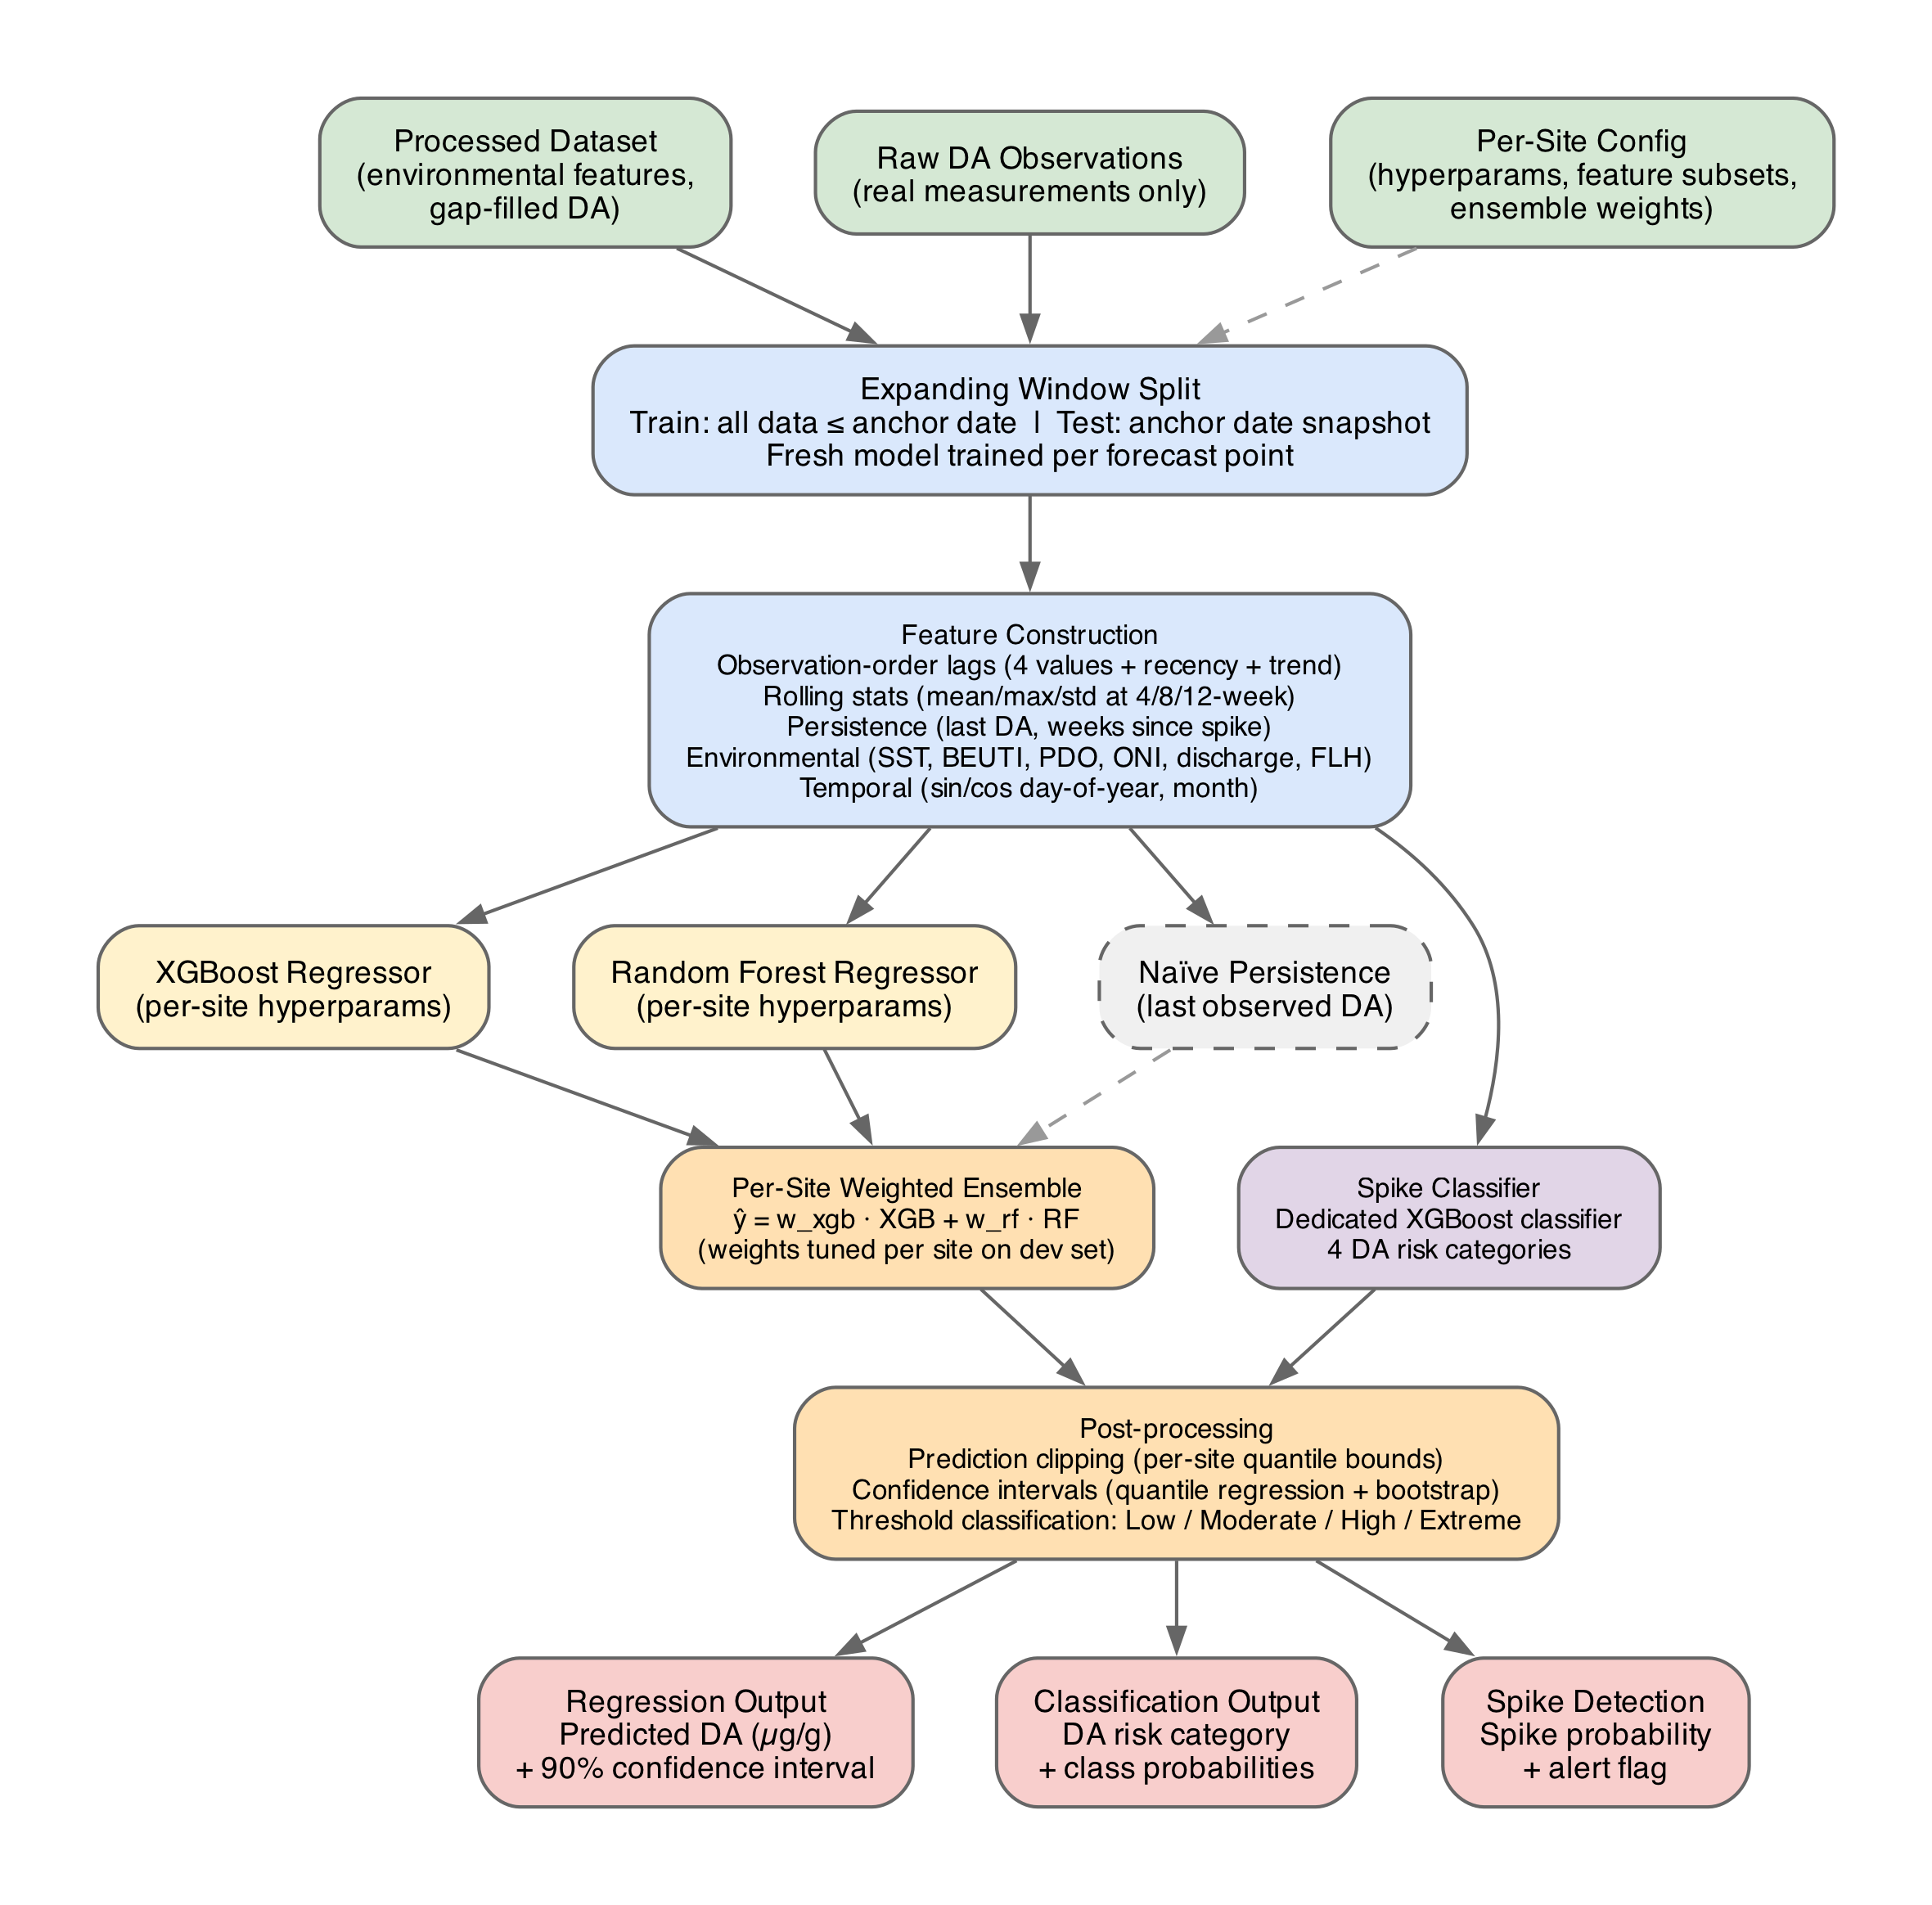
\includegraphics[width=0.85\textwidth]{figures/fig3b_ml_pipeline.png}
\caption{DATect forecasting pipeline: for each forecast point an expanding window enforces chronological splitting at the anchor date and trains a fresh site-specific model, with a separate spike classifier for transition-focused early warning.}
\label{fig:ml-pipeline}
\end{figure}

\subsubsection{Evaluation Metrics}

Regression performance is assessed using the coefficient of determination ($R^2$), mean absolute error (MAE), and root mean squared error (RMSE). Classification performance uses accuracy, per-class precision, recall, and F1 score. For spike detection, three related metrics are used and defined here to avoid ambiguity: \textit{transition recall} is the fraction of below-to-above-threshold crossings (DA crossing from $< \SI{20}{\microgrampeg}$ to $\geq \SI{20}{\microgrampeg}$ relative to the prior observation) correctly identified---the operationally critical metric for early warning; \textit{spike recall} (equivalently, \textit{event recall}) is the fraction of all held-out test rows with DA $\geq \SI{20}{\microgrampeg}$ correctly classified as spikes, regardless of whether a transition occurred. These are evaluated using the F2 score ($\beta = 2$, weighting recall twice as heavily as precision) and a recall-optimized operating point ($p \geq 0.10$), reflecting the asymmetric cost structure where a missed toxic event carries far greater consequence than a false alarm.

\subsection{Web Dashboard Deployment}

DATect is deployed as a publicly accessible web dashboard providing real-time forecasting and retrospective analysis capabilities. Full architectural details, deployment configuration, and visualization descriptions are provided in Appendix~\ref{app:webapp}.


% ══════════════════════════════════════════════════════════════════════════════
%  4. RESULTS
% ══════════════════════════════════════════════════════════════════════════════
\section{Results}
\label{sec:results}

\subsection{Overall Model Performance}
\label{sec:results-overall}

Table~\ref{tab:model-comparison} compares the five model variants evaluated under leak-free retrospective validation on the held-out test set ($n = 2{,}105$). The two-model ML ensemble achieves $R^2 = 0.337$ [95\% CI: 0.257, 0.416], MAE $= \SI{6.53}{\microgrampeg}$, and RMSE $= \SI{19.42}{\microgrampeg}$. Figure~\ref{fig:site-performance} visualizes the site-to-site split that drives this pooled result. Single-seed $R^2$ is noisy (on the post-2022 holdout rows, the 5-seed bootstrap spans 0.29--0.55 across seeds 42--46, std $\approx 0.10$); we therefore caveat all single-number claims with the multi-seed range in Section~\ref{sec:results-temporal-holdout}.

\begin{table}[H]
\caption{Overall regression performance of five model variants under leak-free retrospective validation on the held-out test set ($n = 2{,}105$, seed = 123).}
\label{tab:model-comparison}
\centering\scriptsize
\begin{tabular*}{\linewidth}{@{\extracolsep{\fill}}lcccc}
\toprule
\textbf{Model} & $\boldsymbol{R^2}$ \textbf{[95\% CI]} & \textbf{MAE [CI]} & \textbf{RMSE} & $\boldsymbol{\Delta R^2}$ \textbf{vs.\ ens.} \\
\midrule
\textbf{Per-site sel.}$^{\dagger}$ & \textbf{0.337} [.257, .416] & \textbf{6.53} [5.78, 7.29] & \textbf{19.42} & --- \\
XGBoost          & 0.331 [.257, .410] & 6.78 [6.04, 7.58] & 19.51 & $+$.006 [$-$.006, $+$.017] \\
Random Forest    & 0.330 [.247, .415] & 6.42 [5.67, 7.23] & 19.52 & $+$.007 [$-$.009, $+$.021] \\
Linear (Ridge)   & 0.325 [.242, .410] & 6.61 [5.84, 7.37] & 19.59 & $+$.012 [$-$.007, $+$.032] \\
Na\"ive Persist. & 0.150 [$-$.142, .384] & 6.68 [5.83, 7.60] & 22.00 & $+$.188 [$-$.019, $+$.484] \\
\bottomrule
\end{tabular*}
\vspace{0.3em}\\
\footnotesize{$^\dagger$ Nine of the ten per-site weight pairs are $w \in \{0,1\}$, so ``Per-site selection'' acts mostly as a site-wise model selector (XGBoost at 6 sites, RF at 3; Twin Harbors blends XGBoost 0.25 and RF 0.75); the ensemble formulation is retained for generality (Section~\ref{sec:model-selection}). $\Delta R^2 = R^2_{\text{ens}} - R^2_{\text{comp}}$ (paired bootstrap): positive = ensemble outperforms. MAE in \si{\microgrampeg}.}
\end{table}

The per-site ensemble has the highest point estimate, but XGBoost ($R^2 = 0.331$), Random Forest ($R^2 = 0.330$) and Ridge ($R^2 = 0.325$) are statistically indistinguishable from it: every paired bootstrap difference has a 95\% CI that includes zero (Table~\ref{tab:model-comparison}). Na\"ive persistence reaches $R^2 = 0.150$ with an MAE close to the ensemble's (6.68 vs.\ \SI{6.53}{\microgrampeg}). The ensemble's $R^2$ advantage over persistence is large ($\Delta R^2 = +0.188$) but imprecise ($[-0.019,\, +0.484]$), because a few extreme spikes dominate the pooled squared error; persistence is strong where DA is autocorrelated (Washington; Table~\ref{tab:predictability-ceiling}) and weak where it is not. The models' clearer advantage is in anticipating threshold crossings, which persistence cannot do by construction (Section~\ref{sec:results-spike}).

\subsection{Per-Site Regression Performance}
\label{sec:results-per-site}

Table~\ref{tab:per-site-results} presents detailed per-site ensemble performance. Sites naturally partition into three tiers:

\begin{table}[H]
\caption{Per-site ensemble regression and classification performance on the held-out test set (seed = 123, $n = 2{,}105$), ordered by $R^2$ and grouped into performance tiers.}
\label{tab:per-site-results}
\centering\scriptsize
\begin{tabular*}{\linewidth}{@{\extracolsep{\fill}}lrccrrl}
\toprule
\textbf{Site} & $\boldsymbol{N}$ & $\boldsymbol{R^2}$ \textbf{[95\% CI]} & \textbf{MAE [CI]} & \textbf{RMSE} & \textbf{Acc.} & \textbf{Tier} \\
\midrule
Copalis       & 275 & \textbf{.737} [.649, .824] & 2.15 [1.65, 2.72] & 4.98  & .855 & High \\
Kalaloch      & 222 & \textbf{.603} [.468, .674] & 2.98 [2.10, 4.00] & 7.99  & .865 & High \\
Twin Harbors  & 216 & \textbf{.486} [.359, .768] & 4.67 [2.92, 6.81] & 15.37 & .792 & High \\
Long Beach    & 209 & \textbf{.484} [.354, .656] & 3.71 [2.59, 4.93] & 9.52  & .809 & High \\
Quinault      & 196 & \textbf{.462} [.289, .774] & 3.05 [2.06, 4.33] & 8.67  & .781 & High \\
Clatsop Bch   & 309 & \textbf{.455} [.361, .548] & 5.77 [4.35, 7.48] & 15.30 & .783 & High \\
\addlinespace
Coos Bay      & 110 & .311 [.156, .440] & 24.91 [18.95, 31.42] & 42.20 & .582 & Mod. \\
\addlinespace
Newport       & 208 & .085 [$-$.176, .275] & 11.21 [8.99, 13.73] & 20.30 & .548 & Low \\
Gold Beach    & 242 & .062 [$-$.040, .207] & 12.16 [8.25, 16.77] & 36.18 & .789 & Low \\
Cannon Bch    & 118 & $-$.021 [$-$.070, .145] & 2.72 [1.05, 5.03] & 12.22 & .898 & Low \\
\midrule
\textbf{Overall} & \textbf{2,105} & \textbf{.337} [.257, .416] & \textbf{6.53} [5.78, 7.29] & \textbf{19.42} & \textbf{.778} & --- \\
\bottomrule
\end{tabular*}
\vspace{0.3em}\\
\footnotesize{MAE and RMSE in \si{\microgrampeg}. Bootstrap 95\% CIs ($B = 10{,}000$). Adjusted $R^2$ values differ from $R^2$ by $< 0.02$ at all sites; per-site feature subsetting (Appendix~\ref{app:features}) mitigates modest sample-size-to-feature ratios.}
\end{table}

\begin{table}[H]
\caption{Per-site ensemble performance on the 2022--2023 temporal holdout under two protocols: deterministic chronological (every real DA measurement, $N = 409$) and a 5-seed random-anchor bootstrap (20\% per seed, $N \approx 115$ holdout rows per seed).}
\label{tab:temporal-holdout}
\centering\scriptsize
\begin{tabular*}{\linewidth}{@{\extracolsep{\fill}}lrccrc}
\toprule
\multirow{2}{*}{\textbf{Site}} & \multicolumn{3}{c}{\textbf{Deterministic chronological} (100\% real DA)} & \multicolumn{2}{c}{\textbf{Multi-seed} ($\bar{N}$/seed)} \\
\cmidrule(lr){2-4} \cmidrule(lr){5-6}
              & $\boldsymbol{N}$ & $\boldsymbol{R^2}$ \textbf{[CI]} & \textbf{MAE} & $\boldsymbol{R^2}$ \textbf{mean} $\pm$ \textbf{std} & \textbf{Tier} \\
\midrule
Quinault      & 55  & \textbf{.708} [.518, .832] & 2.96  & .579 $\pm$ .178 & High \\
Coos Bay      & 35  & \textbf{.634} [.451, .869] & 13.84 & .652 $\pm$ .212 & High$^\dagger$ \\
Twin Harbors  & 42  & \textbf{.596} [.342, .755] & 3.82  & .383 $\pm$ .392 & High \\
Copalis       & 60  & \textbf{.589} [.383, .758] & 3.25  & .623 $\pm$ .167 & High \\
Kalaloch      & 35  & \textbf{.537} [.331, .727] & 2.10  & .366 $\pm$ .187 & High \\
Long Beach    & 44  & \textbf{.526} [.204, .843] & 3.63  & .732 $\pm$ .216 & High \\
Clatsop Bch   & 48  & \textbf{.500} [.300, .693] & 5.76  & .466 $\pm$ .209 & High \\
\addlinespace
Newport       & 48  & .041 [$-$.321, .289] & 22.62 & $-$.032 $\pm$ .279 & Low$^\ddagger$ \\
Gold Beach    & 40  & $-$.273 [$-$2.29, .058] & 11.66 & $-$4.19 $\pm$ 5.43 & Low$^\ddagger$ \\
Cannon Bch    & 2   & too few measurements & --- & --- & N/A$^*$ \\
\midrule
\textbf{Overall} & \textbf{409} & \textbf{.419 [.247, .546]} & \textbf{7.49} & \textbf{.377 $\pm$ .105} & --- \\
\bottomrule
\end{tabular*}
\vspace{0.3em}\\
\footnotesize{Deterministic columns: row-level bootstrap CIs ($B = 10{,}000$). MAE in \si{\microgrampeg}. The two protocols measure different kinds of noise: deterministic quantifies which-dates-are-measurable noise; multi-seed quantifies sampling-fraction noise. Multi-seed per-site $N$ is 10--17 holdout rows per seed. $^\dagger$14 of Coos Bay's 35 holdout measurements are spikes, so its $R^2$ rests on a few large events; the MAE of \SI{13.8}{\microgrampeg} reflects that magnitude scale. $^\ddagger$Newport is near zero and Gold Beach negative under both protocols, consistent with their near-zero autocorrelation (Table~\ref{tab:predictability-ceiling}); Gold Beach's multi-seed spread shows how one missed spike dominates $R^2$ at $N \approx 10$. $^*$Cannon Beach has two measurements in 2022--2023.}
\end{table}

\begin{table}[H]
\caption{Persistence-forecast $R^2$ ceiling per site, computed as the squared lag-1 autocorrelation ($\rho^2$) of consecutive raw DA measurements (one per site-day); models with environmental predictors can exceed this persistence-only bound.}
\label{tab:predictability-ceiling}
\centering\small
\begin{tabular*}{\linewidth}{@{\extracolsep{\fill}}lrrrr}
\toprule
\textbf{Site} & $\boldsymbol{N}$ & $\boldsymbol{\rho}$ \textbf{(lag-1)} & $\boldsymbol{R^2}$ \textbf{ceiling} ($\rho^2$) & \textbf{Held-out} $\boldsymbol{R^2}$ \\
\midrule
Copalis       & 687 & 0.901 & 0.813 & 0.737 \\
Kalaloch      & 553 & 0.886 & 0.785 & 0.603 \\
Quinault      & 489 & 0.877 & 0.770 & 0.462 \\
Long Beach    & 522 & 0.854 & 0.730 & 0.484 \\
Twin Harbors  & 538 & 0.852 & 0.726 & 0.486 \\
Clatsop Beach & 772 & 0.840 & 0.705 & 0.455 \\
\addlinespace
Coos Bay      & 273 & 0.505 & 0.255 & 0.311 \\
Cannon Beach  & 293 & 0.481 & 0.232 & $-$0.021 \\
Gold Beach    & 603 & 0.219 & 0.048 & 0.062 \\
Newport       & 518 & 0.218 & 0.047 & 0.085 \\
\bottomrule
\end{tabular*}
\vspace{0.3em}\\
\footnotesize{$N$: measured site-days. $\rho$ computed on consecutive pairs of raw (non-interpolated) measurements at most 28 days apart. WA mean ceiling: 0.765. OR mean ceiling: 0.257. Held-out $R^2$ from Table~\ref{tab:per-site-results} (seed = 123).}
\end{table}

On the all-years paper sample (Table~\ref{tab:per-site-results}, seed = 123, $N = 2{,}105$), the five Washington sites and Clatsop Beach form the \textbf{high-skill} tier with $R^2$ between 0.455 and 0.737; Copalis leads at $R^2 = 0.737$ [0.649, 0.824], and Figure~\ref{fig:pred-vs-obs} illustrates how the ensemble tracks observed DA dynamics at this site over the full 21-year record. Coos Bay ($R^2 = 0.311$) is the \textbf{moderate-skill} tier, while Newport ($R^2 = 0.085$), Gold Beach ($R^2 = 0.062$) and Cannon Beach ($R^2 = -0.021$) form the \textbf{low-skill} tier. The tiers follow the persistence ceiling (Table~\ref{tab:predictability-ceiling}): the six high-skill sites all have $\rho^2 \geq 0.70$, the other four $\rho^2 \leq 0.26$. At Coos Bay, Newport and Gold Beach the held-out $R^2$ exceeds that ceiling, so the environmental features add signal beyond persistence, but at Newport and Gold Beach not enough for useful skill.

The deterministic 2022--2023 holdout evaluation (Table~\ref{tab:temporal-holdout}, $N = 409$ real DA measurements) gives the same picture: the five Washington sites, Clatsop Beach and Coos Bay reach $R^2 = 0.50$--$0.71$; Newport is near zero ($R^2 = +0.041$) and Gold Beach negative ($R^2 = -0.273$) on their near-zero-autocorrelation series; and Cannon Beach has only two measurements in the window, so cannot be evaluated. Eight of the nine evaluable sites are therefore positive on the unbiased holdout. Coos Bay's holdout $R^2$ rests on 35 measurements, 14 of them spikes, and is less stable than its point estimate suggests.

\subsection{Temporal Holdout and Multi-Seed Sensitivity}
\label{sec:results-temporal-holdout}

The 2022--2023 temporal holdout (Table~\ref{tab:temporal-holdout}) provides the strictest unbiased validation: it is downstream of the leak-free grid-search selection window. Two complementary protocols are reported. The \emph{deterministic chronological} evaluation uses every real DA measurement in the holdout window ($N = 409$, 84 spikes), giving a single point estimate per metric with row-level bootstrap CIs: pooled $R^2 = 0.419$ [0.247, 0.546], MAE $= \SI{7.49}{\microgrampeg}$, spike recall $= 0.774$, spike F2 $= 0.693$ (alert at a forecast $\geq \SI{12}{\microgrampeg}$). The complementary \emph{5-seed bootstrap} (20\% random-anchor sampling, $N \approx 115$ holdout rows per seed) quantifies how much single-seed point estimates vary at smaller sample sizes: pooled $R^2 = 0.377 \pm 0.105$ (single-seed range 0.29--0.55). The two estimates are statistically consistent: the deterministic value lies within one inter-seed standard deviation of the multi-seed mean. The standard-eval value of 0.337 (Table~\ref{tab:model-comparison}, single seed 123 from the 40\% random-anchor sample across all years) and the post-2022 holdout numbers are not directly comparable as point estimates---they sample different test sets at different $N$---but the deterministic holdout $R^2$ of $0.419$ is the headline measure of generalization skill. On the 2019--2021 validation window the same evaluation gives $R^2 = 0.329$ [0.203, 0.465] ($N = 635$).

Per site, the multi-seed estimates are much noisier than the deterministic ones because each seed contributes only 10--17 holdout rows per site. The five Washington sites have 5-seed mean $R^2$ between 0.37 and 0.73 with inter-seed std 0.17--0.39. Oregon sites split: Clatsop Beach is comparable to Washington ($0.47 \pm 0.21$), Coos Bay's high apparent $R^2$ ($0.65 \pm 0.21$) rests on $N \approx 10$ per seed, Newport is near zero ($-0.03 \pm 0.28$), and Gold Beach is strongly negative ($-4.2 \pm 5.4$) because a single missed spike dominates $R^2$ at this sample size. Cannon Beach has only two 2022--2023 measurements and cannot be evaluated as a regression target.

The per-site outer configuration (ensemble weights, prediction clip quantile, prediction clip ceiling) was selected by a constrained 3-dimensional grid search tuned strictly on pre-2022 data via chronological 3-fold cross-validation (Limitations item 3). This protocol guarantees that no design decision could have inspected the 2022--2023 holdout. As a defensive check, made before the final data corrections (Section~\ref{sec:retro-eval}), we also ran a prior hand-tuned configuration (selected on a seed-42 development sample across all years) on the same 5-seed bootstrap: hand-tuned scored $R^2 = 0.386 \pm 0.145$ on the holdout versus $0.433 \pm 0.092$ for the grid winners ($\Delta = +0.05 \pm 0.07$, within seed noise), and the hand-tuned configuration scored 0.06 R$^2$ \textit{higher} on the 2019--2022 validation window---the expected signature of the implicit val-window peek in the all-year sampling. Spike-detection metrics (recall and F2) were identical between the two configurations to three decimal places. We retain the grid winners because they require no post-hoc leakage analysis to defend.

\begin{figure}[H]
\centering
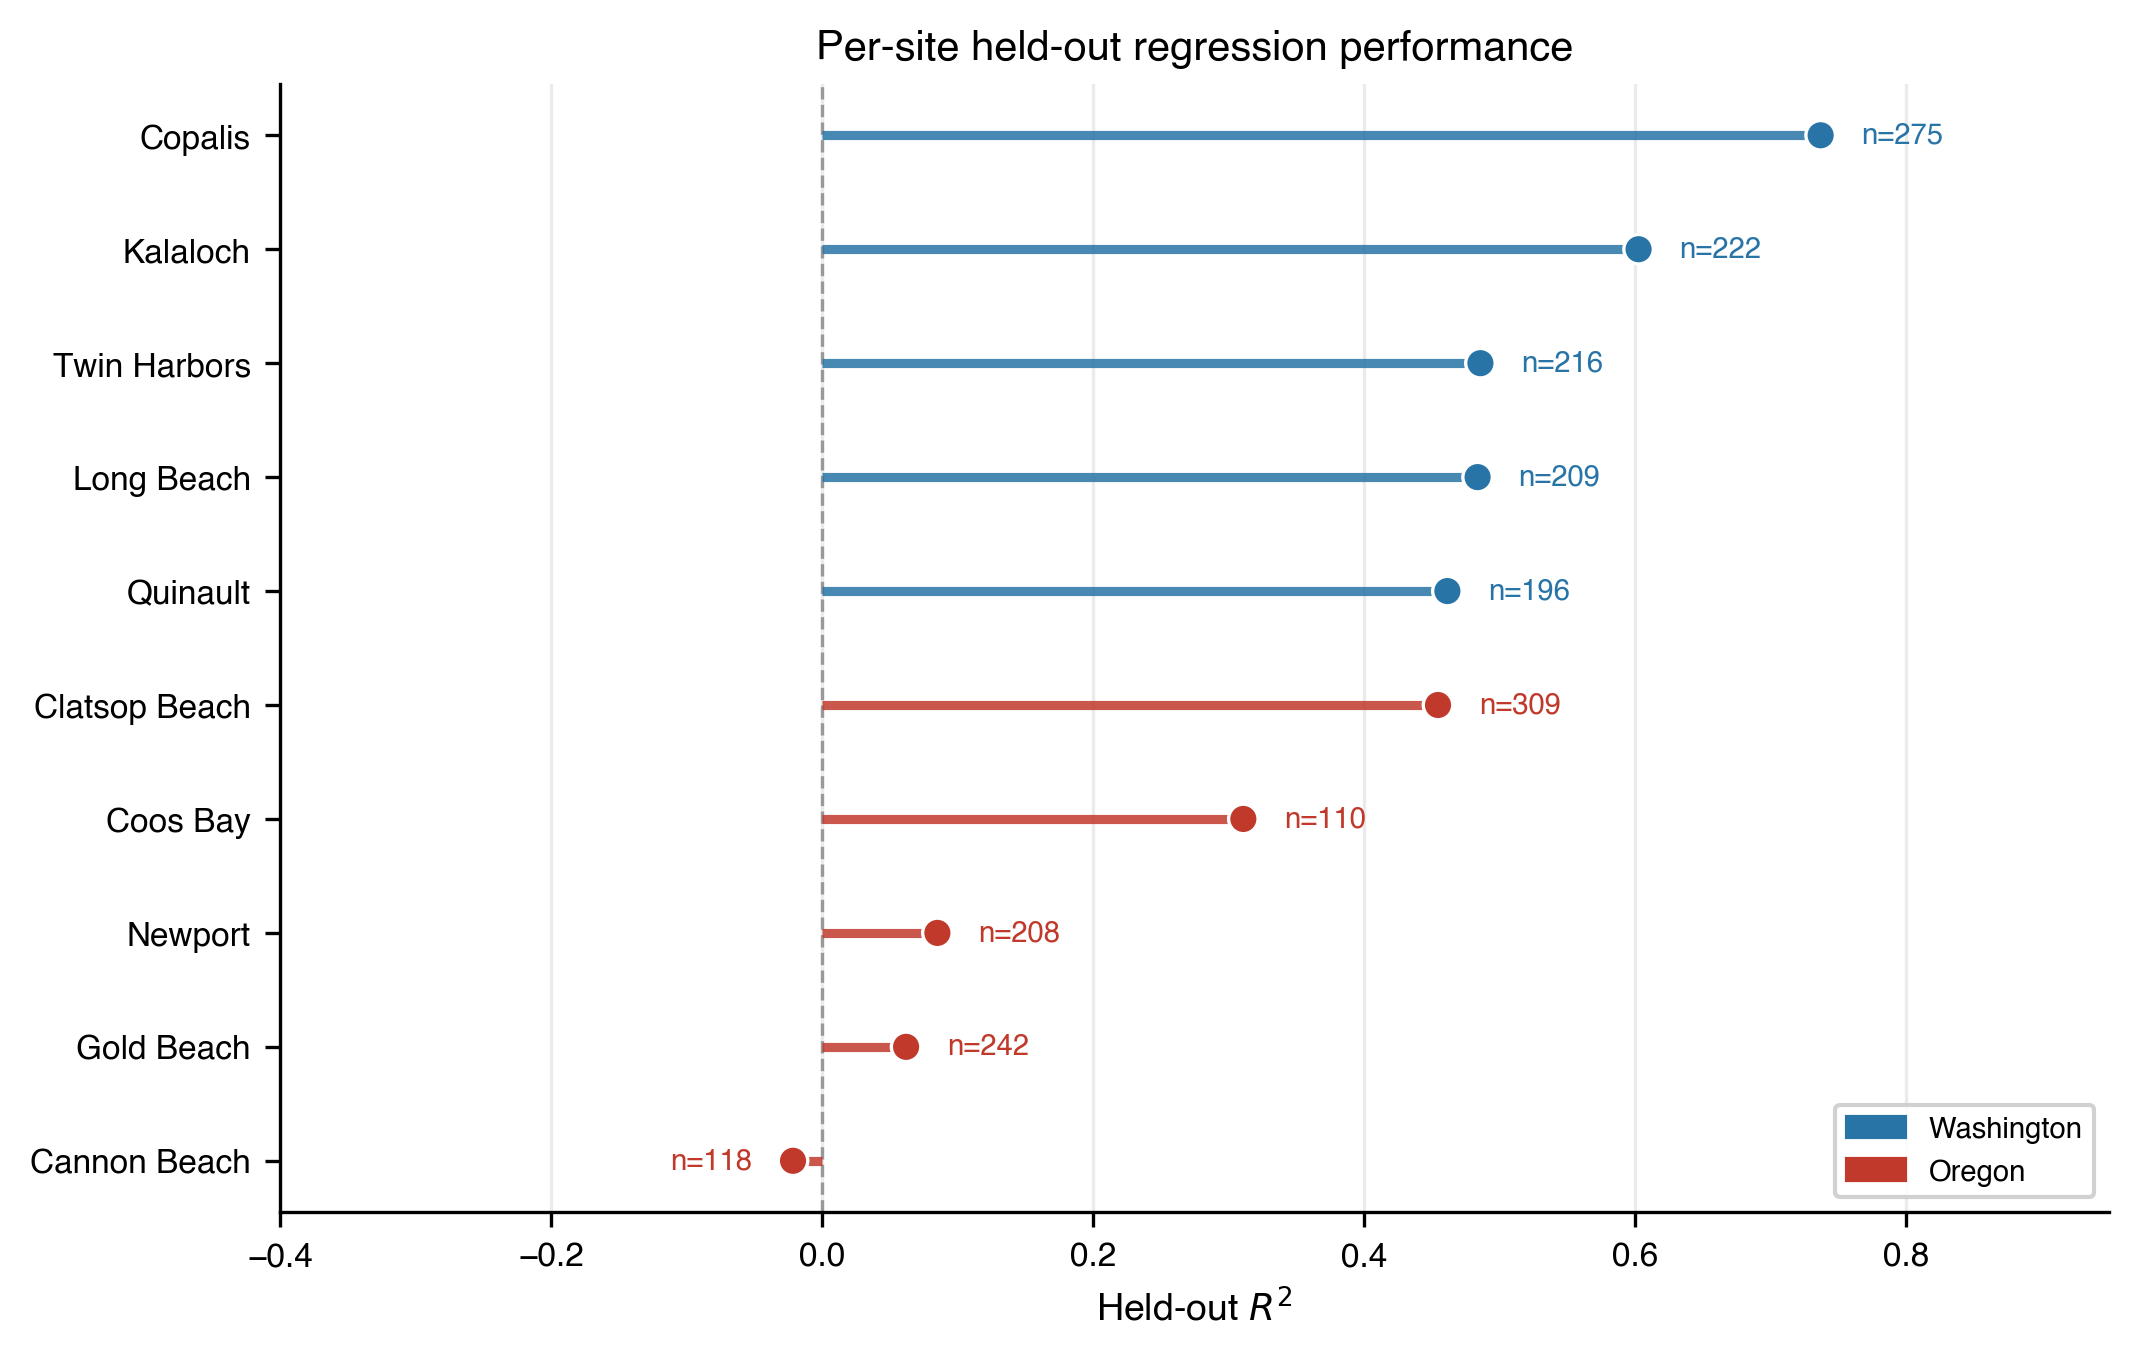
\includegraphics[width=0.9\textwidth]{figures/fig2_site_performance.png}
\caption{Held-out per-site regression performance; Washington sites (blue) outperform Oregon sites (red), and point labels denote the number of validation samples at each site.}
\label{fig:site-performance}
\end{figure}

\begin{figure}[H]
\centering
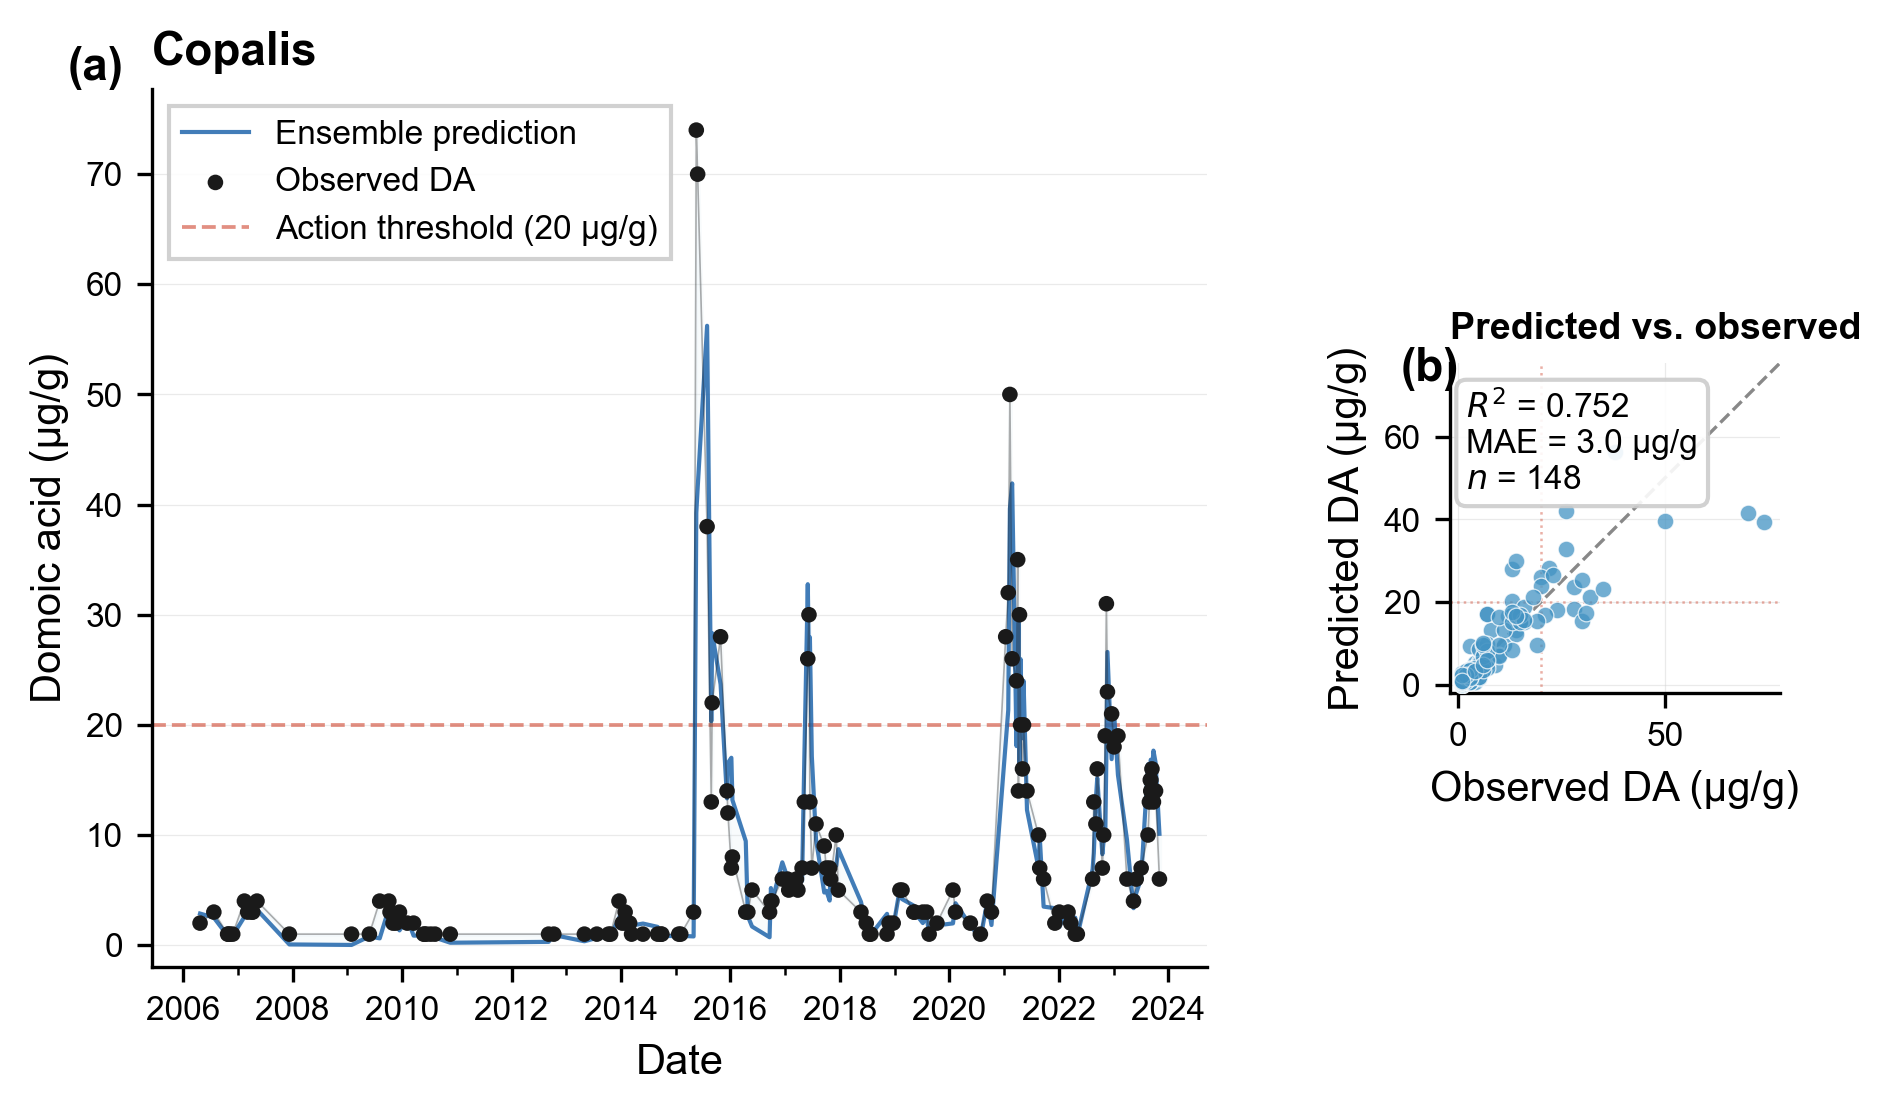
\includegraphics[width=0.9\textwidth]{figures/fig5_pred_vs_obs.png}
\caption{Illustrative ensemble predictions versus observed DA at Copalis (highest-skill site), shown for visualization only: (a) time series over the 21-year record with the \SI{20}{\microgrampeg} FDA threshold; (b) predicted versus observed with the 1:1 line.}
\label{fig:pred-vs-obs}
\end{figure}

\subsection{Classification Performance}
\label{sec:results-classification}

Threshold-based four-category performance is summarized in Appendix~\ref{app:classification-details} (Tables~\ref{tab:classification} and \ref{tab:confusion}). Overall accuracy is 77.8\% on the held-out test set, driven largely by reliable identification of the Low category (F1 $= 0.892$). Higher-risk categories remain more difficult because of limited samples and class imbalance. Most errors occur between adjacent categories, but 11 of 118 Extreme samples (9.3\%) are misclassified as Low---a safety-relevant failure mode that motivates the dedicated spike analysis below and is revisited in Section~\ref{sec:discussion-limitations}.

\subsection{Spike Transition Detection}
\label{sec:results-spike}

While regression metrics characterize average forecasting skill, the operationally critical question is whether DATect can anticipate \emph{spike transitions}---the moment DA crosses from below to at or above the \SI{20}{\microgrampeg} regulatory threshold. These below-to-above crossings are exactly the events that trigger beach closures, and early detection would provide the advance warning that current reactive monitoring cannot. Two distinct event cohorts are used in this section: environmental lead-signal analysis uses all raw-observation threshold crossings identified from consecutive site-level DA measurements (224 events), while forecast evaluation uses only held-out retrospective test rows corresponding to below-to-above-threshold crossings at the same site (93 events, seed = 123).

\subsubsection{Environmental Lead Signals}
\label{sec:results-env-lead}

Analysis of 224 spike transition events across all 10 sites reveals that most environmental features change detectably in the 1--4 weeks \emph{before} DA crosses the regulatory threshold. The largest pre-spike rank-biserial effect sizes (maximum over the four leads) are for SST anomaly ($r = 0.45$), the Pacific Decadal Oscillation (PDO; $r = 0.43$), river discharge ($r = 0.35$, below baseline), SST ($r = 0.30$) and BEUTI ($r = 0.24$); \textit{Pseudo-nitzschia} counts sit below the site baseline before a spike ($r = 0.56$), so their pre-spike signal is a decline rather than a rise. Six of the seven features show \emph{nominal} deviations from baseline ($p < 0.05$, Wilcoxon signed-rank test) at three or more of the four leads; ONI shows none ($p \geq 0.43$ at every lead). A Bonferroni-adjusted familywise threshold of $0.05/7 \approx 0.007$ would be more conservative, and we do not claim simultaneous significance across all tests. This analysis is exploratory---it uses the full dataset, not the held-out test set---and is intended to confirm that pre-spike environmental signal exists in the feature space, not to provide out-of-sample estimates of classifier performance. These lead signals are consistent with the environmental information needed for anticipatory spike detection being present in the feature set.

\subsubsection{Regression Threshold Limitations}
\label{sec:results-threshold-limit}

Despite this, the regression ensemble's spike transition recall at the standard \SI{20}{\microgrampeg} decision threshold is poor: only 8.6\% of held-out transition events (8 of 93) are correctly predicted as spikes (seed = 123). Na\"ive persistence achieves 11.8\%. The ensemble \emph{does} predict elevated values before spikes---mean predicted DA for transition events is \SI{10.8}{\microgrampeg}, against a mean observed \SI{50.2}{\microgrampeg}---but the conservative bias inherent in MSE-optimized regression prevents predictions from crossing the regulatory threshold. A threshold sensitivity analysis confirms this: lowering the decision boundary from 20 to \SI{12}{\microgrampeg} raises overall spike recall from 0.51 to 0.76 while precision falls from 0.74 to 0.57 (this threshold is motivated further in Section~\ref{sec:results-spike-classifier}).

\subsubsection{Transition-Focused Binary Classifier}
\label{sec:results-spike-classifier}

To exploit the pre-spike environmental signals without the regression's conservative bias, we developed a dedicated binary spike classifier, trained as a separate per-anchor model at each retrospective test point. The classifier is an XGBoost model trained on every real DA measurement from all ten sites whose week ends by the anchor (a few thousand rows), with balanced class weights. It excludes the last observed value and the weeks since the last spike but keeps the lagged and rolling DA features, so it learns from both ongoing and new spikes; it is not restricted to below-threshold weeks. The classifier is disabled when fewer than 30 pooled rows or only one class are available.

The deployed \emph{hybrid} alert fires if either the classifier probability exceeds a fixed threshold of $0.10$ or the regression prediction reaches \SI{12}{\microgrampeg}; both are fixed constants in the system configuration (applied identically to every retrospective row). The \SI{12}{\microgrampeg} regression arm is motivated by the systematic under-prediction in the transition band (Section~\ref{sec:results-diagnostics}) and the sensitivity of transition recall to lowering the regression decision boundary (Section~\ref{sec:results-threshold-limit}). Table~\ref{tab:spike-transition} reports metrics on the seed-123 held-out set under this \emph{fixed} policy; we did not optimize these thresholds on that held-out row set to maximize the reported recalls. Absolute recall and precision should therefore be read as conditional on this operating point.

Table~\ref{tab:spike-transition} compares spike transition detection across approaches on the held-out retrospective panel (seed = 123, $n = 2{,}105$, 278 spikes, 93 below-to-above-threshold transitions). Figure~\ref{fig:spike-summary} shows the same operating-point tradeoff.

\begin{table}[H]
\caption{Spike transition detection performance on the held-out retrospective panel ($n = 2{,}105$, 93 below-to-above-threshold transitions; seed = 123), each approach evaluated at its own canonical alert threshold.}
\label{tab:spike-transition}
\centering\footnotesize
\begin{tabular*}{\linewidth}{@{\extracolsep{\fill}}lcccc}
\toprule
\textbf{Approach} & \textbf{Trans.\ Rec.} & \textbf{Spike Rec.} & \textbf{Prec.} & \textbf{F2} \\
\midrule
Na\"ive persistence ($\geq$20 \si{\microgrampeg})        & 0.118 & 0.701 & 0.666 & 0.694 \\
Ensemble ($\geq$20 \si{\microgrampeg})                  & 0.086 & 0.511 & 0.736 & 0.544 \\
Spike classifier ($p \geq 0.10$)                         & 0.731 & 0.910 & 0.483 & 0.773 \\
Hybrid alert (cls.\ $\cup$ regression $\geq$12 \si{\microgrampeg}) & \textbf{0.763} & \textbf{0.921} & 0.474 & \textbf{0.775} \\
\bottomrule
\end{tabular*}
\vspace{0.3em}\\
\footnotesize{F2 weights recall twice as heavily as precision ($\beta = 2$). The hybrid's advantage is concentrated in \textit{transition} recall (0.763 vs.\ 0.118, a 6.5$\times$ improvement), which F2 does not separately capture.}
\end{table}

\begin{figure}[H]
\centering
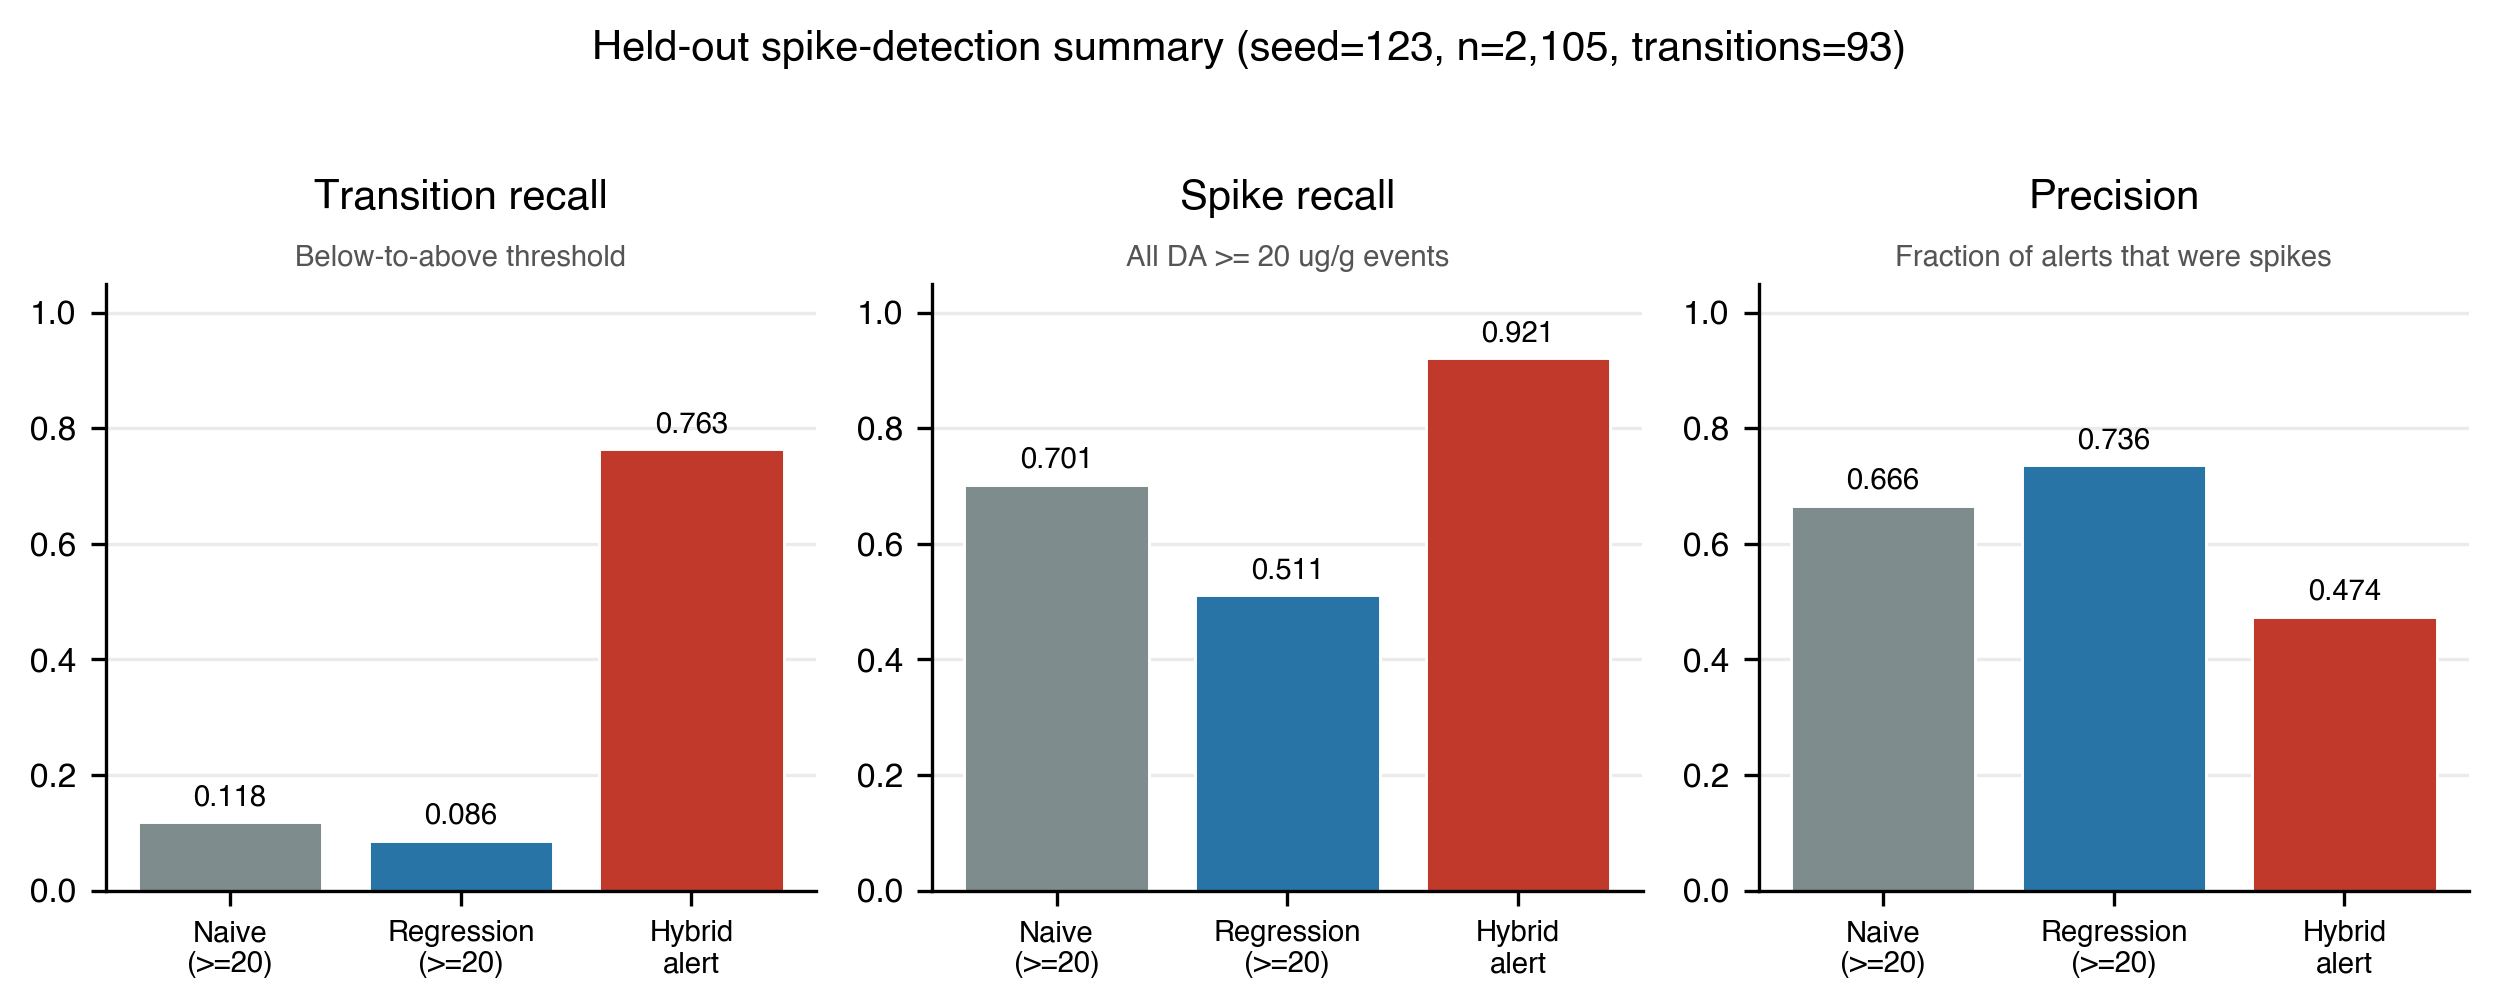
\includegraphics[width=0.88\textwidth]{figures/fig4_spike_detection_summary.png}
\caption{Spike-focused summary of the held-out results in Table~\ref{tab:spike-transition}.}
\label{fig:spike-summary}
\end{figure}

The hybrid alert---combining the transition-focused classifier with a regression trigger at \SI{12}{\microgrampeg}---achieves 76.3\% transition recall compared to 11.8\% for na\"ive persistence (at the \SI{20}{\microgrampeg} regulatory threshold) and 8.6\% for the standard regression ensemble. This 6.5$\times$ improvement in transition recall over na\"ive persistence comes at the cost of lower precision (0.474 hybrid vs.\ 0.666 naive), roughly one false alarm per true alert. Because F2 weights recall twice as heavily as precision, the hybrid's overall F2 (0.775) still exceeds na\"ive persistence (0.694). The classifier alone captures most of this (transition recall 0.731); the regression arm at \SI{12}{\microgrampeg} adds three more onsets. On the deterministic 2022--2023 holdout ($N = 409$, 29 transitions) the hybrid alert detects 89.3\% of spikes and 20 of the 29 onsets (69.0\%). The classifier's top feature is the rolling DA maximum over 4 weeks (normalized gain importance 0.31--0.34 across the five bootstrap seeds 42--46, averaged over 60 retraining anchors per seed); the 4-, 8- and 12-week rolling maxima together carry 57\% of the gain, consistent with the biological mechanism where gradual toxin accumulation precedes a threshold crossing. Environmental features contribute far less: PDO is the strongest (0.03), and ONI, BEUTI, fluorescence, discharge and SST each stay near 0.01.

\subsection{Ablation Study}
\label{sec:results-ablation}

Component ablation is summarized in Appendix~\ref{app:component-ablation} (Table~\ref{tab:ablation}), evaluated on the development sample (seed = 42, 20\%, $n = 1{,}054$) under the current grid-winner per-site configuration. On the corrected targets no single component changes $R^2$ by more than 0.01. Removing the per-site configuration costs $\Delta R^2 = -0.005$, but this nets out two opposing effects that the perturbation study separates (Table~\ref{tab:perturbation}): the per-site clip quantiles now truncate real spikes (relaxing them to the global 0.99 gains $+0.039$), while the per-site weights and hyperparameters still add roughly 0.04 relative to the global defaults. Dropping the gap-filled training rows raises $R^2$ slightly ($+0.007$) but also raises MAE (6.29 to \SI{6.39}{\microgrampeg}), so the gap-fill is neutral on this sample. Observation-order lags ($+0.003$ when removed) and the derived \texttt{pn\_log} ($+0.000$) show negligible standalone impact at the one-week horizon, consistent with redundancy with the persistence and rolling-statistics features. The OAD ocean-anomaly features are likewise sub-noise ($+0.003$ when removed) for reasons discussed in Section~\ref{sec:discussion-feature-extension}.

\begin{sloppypar}
The feature-group ablation (Appendix~\ref{app:feature-ablation}, Table~\ref{tab:feature-ablation}) shows that no group of environmental predictors exceeds noise-level impact ($|\Delta R^2| \leq 0.004$), and removing all of them at once costs only $\Delta R^2 = -0.004$. Feature importance rankings (Figure~\ref{fig:feature-importance}) show that DA-history features (\texttt{last\_observed\_da\_raw}, \texttt{weeks\_since\_last\_spike}, observation-order lags and rolling statistics) account for 53\% of total model gain, the 16 OAD features for 34\%, and the climate, satellite, upwelling, discharge and \textit{Pseudo-nitzschia} predictors together for 8\%. High gain importance does not imply marginal contribution: the trees split on the OAD features often, yet removing them changes $R^2$ by only $+0.003$, so they carry no information the other features lack. The perturbation study (Appendix~\ref{app:perturbation-sensitivity}, Tables~\ref{tab:perturbation}--\ref{tab:seed-stability}) shows that RF hyperparameters and monotonic constraints are insensitive, that model-family and feature-subset choices stay within 0.015, and that Washington sites are stable across five seeds (mean $R^2$ 0.41--0.78), with Oregon variance reflecting data scarcity rather than tuning fragility.
\end{sloppypar}


\subsection{Diagnostic Findings}
\label{sec:results-diagnostics}

Two diagnostic analyses characterize where the ensemble fails. An episodic-error decomposition on the seed-123 sample shows that 90.6\% of total squared error concentrates in the worst 5\% of test rows ($n = 105$). Most of these are at Oregon sites (82\%, chiefly Coos Bay, Gold Beach and Newport) and most are under-predicted extreme events (76\% have observed DA $\geq \SI{40}{\microgrampeg}$), consistent with the low autocorrelation ceilings at those sites (Table~\ref{tab:predictability-ceiling}). A bias analysis in the 12--30~\si{\microgrampeg} transition zone ($n = 273$ observations) reveals a systematic under-prediction of \SI{4.8}{\microgrampeg} (mean observed minus predicted), a predictable consequence of MSE-optimized regression on a right-skewed target and the primary motivation for the hybrid alert's transition-focused classifier.

% ══════════════════════════════════════════════════════════════════════════════
%  5. DISCUSSION
% ══════════════════════════════════════════════════════════════════════════════
\section{Discussion}
\label{sec:discussion}

\subsection{Data Quality and Site Heterogeneity}

The clearest pattern in the held-out results is a gradient from the Washington coast and the Columbia River mouth (Clatsop Beach) to the southern Oregon sites. As reported in Section~\ref{sec:results-per-site}, 8 of the 9 evaluable sites are positive on the 2022--2023 deterministic holdout, with 7 in $R^2 = 0.50$--$0.71$. The strongly negative per-site values under the multi-seed protocol (Gold Beach $-4.2 \pm 5.4$) are largely small-per-seed-$N$ amplification: at $N \approx 10$ per site per seed, a single mispredicted spike week can dominate the residual sum and crush the per-site $R^2$. Under the deterministic protocol at $N \approx 40$ per site, Newport is near zero and only Gold Beach remains negative.

The gradient follows the persistence ceiling more closely than the state line: Clatsop Beach has Washington-like autocorrelation ($\rho^2 = 0.71$) and skill, while Newport and Gold Beach have $\rho^2 \approx 0.05$ (Table~\ref{tab:predictability-ceiling}). One plausible contributor is data quality: Washington records from WDFW and Tribal monitoring are denser and more temporally regular, so persistence, lag, and rolling features can be estimated more reliably. Oregon records are sparser and less regular, reducing the effective information content available to both linear and nonlinear models. Genuine oceanographic differences may also contribute: Washington beaches are influenced by the Juan de Fuca eddy and the Columbia River plume, both of which may increase DA persistence or provide stronger environmental structure \cite{Trainer2009, McCabe2023}. Even so, monitoring density is likely the primary constraint on forecast skill, and better-sampled Oregon records would likely improve performance more than a more complex model family.

\subsection{Persistence, Model Choice, and ML Contribution}

The difference between the standard single-seed paper sample ($R^2 = 0.337$ at seed = 123, all-years) and the post-2022 deterministic holdout ($R^2 = 0.419$ on $N = 409$ real DA measurements in 2022--2023) is worth interpreting. First, the windows differ: the paper sample mixes all years 2003--2023, including periods with sparse Oregon coverage; the deterministic holdout is restricted to 2022--2023 when monitoring was relatively dense. Second, the paper sample is a single 40\% draw at one seed; the deterministic holdout uses every real DA measurement in the window. Across the two protocols on the post-2022 window, Washington sites fall in the $R^2 = 0.53$--$0.71$ range on the deterministic protocol and $0.37$--$0.73$ on the 5-seed bootstrap. These ranges agree within bootstrap CI: tuned configurations generalize where data quality permits, and the lower aggregate single-seed $R^2 = 0.337$ on the paper sample reflects the low-skill southern Oregon sites and small per-site $N$, not overfitting. The 5-seed bootstrap on the post-2022 holdout rows (Table~\ref{tab:temporal-holdout}) confirms this: across seeds 42--46, pooled $R^2$ ranges 0.29--0.55 with mean $0.377 \pm 0.105$, consistent with the deterministic point estimate.

Strong persistence at several Washington sites is biologically plausible. DA depuration from razor clam tissue occurs over weeks to months \cite{Drum1993, Wekell1994}, so one-week-ahead DA often remains close to the most recent observation during sustained bloom periods. DATect therefore treats na\"ive persistence as a serious external baseline rather than a straw man. Its pooled held-out $R^2$ of 0.150, well below the ensemble's 0.337 but with an overlapping CI, reflects that persistence is highly site-dependent: strong where DA is autocorrelated, and close to useless at Newport and Gold Beach.

The near-tie between the tree-based models and Ridge regression further shows that most forecast signal comes from the feature set, above all the DA history, not from an intrinsically superior model family. On the corrected targets the per-site configuration is roughly neutral in aggregate ($\Delta R^2 = -0.005$ when removed; Table~\ref{tab:ablation}): its tuned weights and hyperparameters help, but its clip quantiles, selected against the uncorrected targets, now cost a similar amount (Appendix~\ref{app:perturbation-sensitivity}). Likewise, model-selection robustness in Appendix~\ref{app:weight-robustness} shows that choosing XGBoost versus Random Forest per site changes aggregate $R^2$ only modestly.

This perspective also helps interpret the ablations. Gap-filled training rows are neutral on the development sample, while observation-order lags and derived features show little standalone marginal effect at the one-week horizon---their signal overlaps with persistence and rolling-history terms, and tree models can capture simple nonlinear structure without handcrafted interactions.

\subsection{Spike Detection and Management Relevance}
\label{sec:discussion-spike}

The spike results reveal a different operational problem from regression accuracy. The regression ensemble's spike recall at the operationally-tuned \SI{12}{\microgrampeg} alert threshold reaches 0.774 on the deterministic 2022--2023 holdout (Table~\ref{tab:temporal-holdout}), but thresholding at the regulatory \SI{20}{\microgrampeg} limit catches only a small fraction of held-out below-to-above-threshold transitions even though the model often predicts elevated pre-spike values (Section~\ref{sec:results-spike}). This is a predictable consequence of MSE-optimized regression on an imbalanced target: the model is rewarded for shrinking extreme values toward the center of the distribution. For closure-relevant early warning, that conservative bias is a feature for average error but a liability for threshold crossings.

The transition-focused classifier addresses that failure mode by changing the task definition, relying on environmental precursors and gradual toxin accumulation rather than simple persistence (Section~\ref{sec:results-spike-classifier}). The hybrid alert (classifier $\cup$ regression trigger at \SI{12}{\microgrampeg}) yields a substantial increase in transition recall over na\"ive persistence, at the cost of lower precision than either component alone. This tradeoff is appropriate for a decision-support system: a false alert increases sampling attention, whereas a missed transition can leave managers reacting only after DA has crossed the regulatory limit.

That distinction matters for management value. Quantitative one-week forecasts can support precautionary advisories, sampling prioritization, and more informed timing of openings and closures. The existing PNW HAB Bulletin already provides measurable value through qualitative expert advisories \cite{Jin2024}; DATect complements that workflow with explicit numerical forecasts and a transition-focused alert channel, delivered through a publicly accessible web dashboard (Appendix~\ref{app:webapp}) that supports both real-time forecasting and retrospective analysis across all 10 sites.

\subsection{Limitations}
\label{sec:discussion-limitations}

\begin{enumerate}[nosep]
    \item \textbf{Per-site skill on the small-$N$ Oregon coast}: On the single-seed paper sample (Table~\ref{tab:per-site-results}, all years), Newport, Gold Beach and Cannon Beach have $R^2$ near zero ($-0.02$ to $0.09$) and Coos Bay is moderate (0.31). On the deterministic post-2022 holdout (Table~\ref{tab:temporal-holdout}), Coos Bay and Clatsop Beach reach $R^2 \approx 0.5$--$0.6$, Newport is near zero ($+0.04$), and Gold Beach is negative ($R^2 = -0.27$). Cannon Beach has only two measurements in the 2022--2023 window and is not evaluable. The lag-1 autocorrelation analysis (Table~\ref{tab:predictability-ceiling}) gives persistence-forecast $R^2$ ceilings of 0.05 for Newport and Gold Beach and 0.23--0.26 for Cannon Beach and Coos Bay, so consecutive DA measurements at these sites carry little information about the next observation. This does not preclude improvement from environmental predictors---Coos Bay, Newport and Gold Beach all exceed their persistence ceilings (e.g., Coos Bay $R^2 = 0.311 > \rho^2 = 0.255$)---but the low autocorrelation structure means persistence-based signal contributes little. The paper cannot fully separate data sparsity from true regional oceanographic complexity; denser Oregon monitoring records and richer environmental predictors may yet reveal exploitable structure currently obscured by irregular sampling.
    \item \textbf{High-risk category weakness}: The High and Extreme DA categories remain difficult, with F1 scores of 0.404 and 0.448, and 9.3\% of Extreme events are misclassified as Low under threshold-based four-category classification.
    \item \textbf{Per-site outer configuration is selected by leak-free grid search}: The per-site values in \texttt{per\_site\_models.py} (ensemble weights, prediction clip quantile, prediction clip ceiling) were selected by a constrained 3-dimensional grid search (75 configurations per site) tuned strictly on pre-2022 data via chronological 3-fold cross-validation (folds: 2019, 2020, 2021); the 2022--2023 holdout window was never inspected during selection. The defensive comparison against the prior hand-tuned configuration (Section~\ref{sec:results-temporal-holdout}) showed a small validation-window leak in the all-year hand-tuning that reversed on the holdout, within seed noise; we retain the grid-search winners because they remove the indirect-leak concern by construction. That search, however, was run before the evaluation targets were corrected to one measurement per site-day (Section~\ref{sec:retro-eval}). Against the corrected targets the selected clip quantiles truncate real spikes (on the development sample, $R^2$ rises from 0.332 to 0.388 without clipping; Table~\ref{tab:perturbation}), so the grid search must be re-run on the corrected data, and checked once on the holdout, before the per-site configuration can be considered final. A more aggressive 18-dimensional Optuna search over per-anchor XGB and Random Forest hyperparameters using the same protocol produced gains on the validation window ($+0.07$ R$^2$) that fully reversed on the holdout ($-0.16$ R$^2$), indicating the model is feature-limited rather than hyperparameter-limited under broader search.
    \item \textbf{Uncertainty summaries are not full probabilistic guarantees}: The quantile bands used for forecasts are hybrid empirical intervals, and the bootstrap confidence intervals reported for retrospective metrics resample held-out prediction rows with replacement (Section~\ref{sec:validation}). They summarize variability across the sampled test rows under that scheme; they are not block-bootstrap intervals over time or space and do not establish exact calibration under temporal or spatial dependence.
    \item \textbf{Operational deployment remains simplified}: The current system relies on pre-computed cache and a seven-day forecast horizon aligned with the PNW HAB Bulletin. Real-time ingestion and longer forecast horizons remain open engineering and scientific challenges.
    \item \textbf{Sensor continuity}: MODIS-Aqua is approaching end of life, so future operational use will require careful recalibration to successor instruments such as PACE.
\end{enumerate}

\subsection{Feature-Extension Experiments and the Data-Limited Ceiling}
\label{sec:discussion-feature-extension}

To test whether the current feature set is at its data-limited ceiling, we ran six independent feature-extension ablations using the same leakage-controlled A/B retrospective protocol: (i) lagged \textit{Pseudo-nitzschia} cell-count statistics, (ii) BEUTI nonlinear derivatives, (iii) NEMO regional mooring anomalies, (iv) ESP offshore particulate-DA measurements, (v) NDBC 46041 wind upwelling-stress proxies, and (vi) a 16-dimensional regional ocean-anomaly representation produced from an unsupervised 3D masked autoencoder over 22 years of MODIS Aqua imagery (Chen et al., in preparation). All six were null at the pooled level with $|\Delta R^2| < 0.003$, well inside the multi-seed bootstrap noise floor. The autoencoder result is the most informative: the learned representation validates strongly against in-situ ESP mooring measurements at the offshore source (Pearson $r = +0.46$ vs.\ \textit{Pseudo-nitzschia} cell counts, $r = +0.33$ vs.\ particulate DA), yet contributes zero net skill at the beach DA level (\(\Delta\) R$^2 = +0.002$ across all 10 sites). The signal does not survive the variable wind-driven onshore transport (~24 km) and subsequent 1--2 week razor clam bioaccumulation chain. Together with the failed hyperparameter tuning, these results support the interpretation that DATect's residual error is dominated by stochasticity in the offshore-to-shore-to-shellfish causal chain plus monitoring sparsity, not by inadequate model capacity.

\subsection{Future Work}
\label{sec:discussion-future}

The highest-impact next step is improved Oregon monitoring. If data quality is the binding constraint, then denser and more regular sampling should produce larger gains than architecture changes alone. Transfer learning or hierarchical models could help in the interim, but they are unlikely to substitute fully for missing observations.

Additional gains may come from richer observing systems. PACE hyperspectral ocean color \cite{Werdell2019} could improve satellite characterization of bloom conditions, while offshore molecular measurements \cite{Brunson2024} could provide more direct evidence of toxigenic \textit{Pseudo-nitzschia} activity. Sequence models or spatial along-coast models may also become more attractive once the observational record is dense enough to support them.


% ══════════════════════════════════════════════════════════════════════════════
%  6. CONCLUSIONS
% ══════════════════════════════════════════════════════════════════════════════
\section{Conclusions}
\label{sec:conclusions}

DATect provides the first quantitative one-week-ahead domoic acid forecasting system for Washington and Oregon. Under a leak-free 3-window chronological evaluation, the per-site ensemble achieves pooled $R^2 = 0.419$ [95\% CI: 0.247, 0.546] on the 2022--2023 temporal holdout ($N = 409$ deterministic, all real DA measurements; consistent 5-seed bootstrap confirmation $R^2 = 0.377 \pm 0.105$). Eight of the 9 evaluable sites achieve positive holdout skill; 7 sites fall in the $R^2 = 0.50$--$0.71$ band, including all five Washington sites and two Oregon sites (Clatsop Beach, Coos Bay). The resulting scientific message is not simply that DATect can forecast DA, but that regional monitoring quality currently places the strongest upper bound on forecast skill.

The paper's main operational result is that magnitude forecasting and closure-warning are related but distinct tasks. Regression-only spike recall reaches 0.774 at the \SI{12}{\microgrampeg} threshold on the deterministic holdout, but thresholding the regression ensemble at \SI{20}{\microgrampeg} catches only a fraction of the below-to-above-threshold transitions that trigger harvest closures, because MSE-optimized regression conservatively under-predicts extremes (Section~\ref{sec:results-spike}). A dedicated transition-focused classifier substantially improves transition recall, and the resulting hybrid alert (classifier $\cup$ regression trigger) detects 92.1\% of spikes and 76.3\% of new spike onsets on the retrospective panel, against 11.8\% of onsets for na\"ive persistence. DATect therefore contributes both a quantitative forecasting pipeline and a transition-focused early-warning layer that can complement the qualitative PNW HAB Bulletin, with the entire tuning workflow (per-site configurations, evaluation windows, classifier thresholds) reproducible end-to-end from a single source-of-truth JSON file.


% ══════════════════════════════════════════════════════════════════════════════
%  ACKNOWLEDGMENTS
% ══════════════════════════════════════════════════════════════════════════════
\vspace{6pt}

\authorcontributions{Conceptualization, A.C.; methodology, A.C.; software, A.C.; validation, A.C.; formal analysis, A.C.; investigation, A.C.; data curation, A.C.; writing---original draft preparation, A.C.; writing---review and editing, A.C.\ and J.M.; visualization, A.C.; supervision, J.M. All authors have read and agreed to the published version of the manuscript.}

\funding{This research received no external funding.}

\institutionalreview{Not applicable.}

\informedconsent{Not applicable.}

\dataavailability{The DATect source code and web dashboard are available at \url{https://github.com/ansoncchen/DATect-Forecasting-Domoic-Acid}. Processed datasets and pre-computed cache files are available upon reasonable request.}

\acknowledgments{DA measurement data were provided by the Washington Department of Health, Washington Department of Fish and Wildlife, Oregon Department of Fish and Wildlife, and the Olympic Region Harmful Algal Bloom (ORHAB) Partnership. Satellite data were obtained from the NOAA CoastWatch ERDDAP server. Climate index data were obtained from NOAA ERDDAP. Columbia River discharge data were obtained from the U.S.\ Geological Survey. Computational resources were provided by the University of Washington Hyak high-performance computing cluster.}

\conflictsofinterest{The authors declare no conflict of interest.}


% ══════════════════════════════════════════════════════════════════════════════
%  APPENDICES
% ══════════════════════════════════════════════════════════════════════════════
\appendix
\appendixstart

\section{Per-Site Model Configuration}
\label{app:model-config}

Table~\ref{tab:ensemble-config} summarizes the site-wise model weights and clipping rules selected by the leak-free grid search (Section~\ref{sec:results-temporal-holdout}), with each site's held-out performance tier.

\begin{table}[H]
\caption{Per-site ensemble configuration (grid-search winners in \texttt{config/tuned\_hyperparameters.json}) and held-out performance tier from Table~\ref{tab:per-site-results}.}
\label{tab:ensemble-config}
\centering\footnotesize
\begin{tabular*}{\linewidth}{@{\extracolsep{\fill}}lcccrl}
\toprule
\textbf{Site} & $\boldsymbol{w_{\text{XGB}}}$ & $\boldsymbol{w_{\text{RF}}}$ & \textbf{Clip $q$} & \textbf{Clip max} & \textbf{Tier} \\
\midrule
Copalis       & 1.00 & 0.00 & 0.97 & --- & High \\
Kalaloch      & 0.00 & 1.00 & 0.95 & --- & High \\
Twin Harbors  & 0.25 & 0.75 & 0.97 & --- & High \\
Long Beach    & 1.00 & 0.00 & 0.95 & --- & High \\
Quinault      & 1.00 & 0.00 & 0.95 & --- & High \\
Clatsop Bch   & 1.00 & 0.00 & 0.95 & --- & High \\
\addlinespace
Coos Bay      & 0.00 & 1.00 & 0.95 & --- & Mod. \\
\addlinespace
Newport       & 1.00 & 0.00 & 0.95 & --- & Low \\
Gold Beach    & 1.00 & 0.00 & 0.97 & --- & Low \\
Cannon Bch    & 0.00 & 1.00 & 0.95 & --- & Low \\
\bottomrule
\end{tabular*}
\vspace{0.3em}\\
\footnotesize{Clip~$q$: predictions clipped to this quantile of training targets. ``---'' = no hard ceiling (the global default quantile, used when a site sets none, is $q = 0.99$). Clip max in \si{\microgrampeg}. Model-family choice changes pooled skill little (Appendix~\ref{app:weight-robustness}).}
\end{table}

\section{Classification Details}
\label{app:classification-details}

\begin{table}[H]
\caption{DA risk categories used in DATect classification.}
\label{tab:da-categories}
\centering\small
\begin{tabularx}{\linewidth}{lcX}
\toprule
\textbf{Category} & \textbf{DA Range (\si{\microgrampeg})} & \textbf{Interpretation} \\
\midrule
Low      & 0--5   & Safe for harvest \\
Moderate & 5--20  & Monitor closely \\
High     & 20--40 & Elevated toxicity; closures likely \\
Extreme  & $\geq$40  & Dangerous; immediate closure \\
\bottomrule
\end{tabularx}
\end{table}

\begin{table}[H]
\caption{Per-category classification performance on the held-out test set ($n = 2{,}105$). Categories are left-closed: a value of exactly \SI{20}{\microgrampeg} is High.}
\label{tab:classification}
\centering\small
\begin{tabular*}{\linewidth}{@{\extracolsep{\fill}}lrrrrr}
\toprule
\textbf{Category} & \textbf{DA Range} & $\boldsymbol{N}$ & \textbf{Precision} & \textbf{Recall} & \textbf{F1} \\
\midrule
Low      & 0--5 \si{\microgrampeg}  & 1{,}370 & 0.871 & 0.914 & 0.892 \\
Moderate & 5--20 \si{\microgrampeg} & 457 & 0.603 & 0.626 & 0.614 \\
High     & 20--40 \si{\microgrampeg} & 160 & 0.438 & 0.375 & 0.404 \\
Extreme  & $\geq$40 \si{\microgrampeg}  & 118 & 0.696 & 0.331 & 0.448 \\
\midrule
\multicolumn{2}{l}{\textbf{Overall (macro)}} & \textbf{2,105} & \textbf{0.652} & \textbf{0.561} & \textbf{0.590} \\
\multicolumn{2}{l}{Overall accuracy} & & \multicolumn{3}{r}{77.8\%} \\
\bottomrule
\end{tabular*}
\end{table}

\begin{table}[H]
\caption{Confusion matrix for four-category DA classification.}
\label{tab:confusion}
\centering\small
\begin{tabular*}{\linewidth}{@{\extracolsep{\fill}}lrrrr}
\toprule
\textbf{Actual \textbackslash\ Predicted} & \textbf{Low} & \textbf{Moderate} & \textbf{High} & \textbf{Extreme} \\
\midrule
Low      & 1252 & 83  & 24 & 11 \\
Moderate & 155  & 286 & 15 & 1 \\
High     & 20   & 75  & 60 & 5 \\
Extreme  & 11   & 30  & 38 & 39 \\
\bottomrule
\end{tabular*}
\end{table}

\section{Component Ablation}
\label{app:component-ablation}

\begin{table}[H]
\caption{Component ablation: each row removes one component from the full DATect system, evaluated on the development sample (seed = 42, 20\%, $n = 1{,}054$).}
\label{tab:ablation}
\centering\footnotesize
\begin{tabularx}{\linewidth}{lcccX}
\toprule
\textbf{Configuration} & $\boldsymbol{R^2}$ & $\boldsymbol{\Delta R^2}$ & \textbf{MAE} & \textbf{Notes} \\
\midrule
Full DATect (baseline)    & 0.332 & ---      & 6.29 & Grid-winner per-site config \\
No per-site custom.       & 0.327 & $-$0.005 & 6.14 & Equal XGB/RF weights, global hyperparameters, all features, clip $q = 0.99$ \\
No interp.\ training      & 0.339 & +0.007 & 6.39 & Real DA rows only as training targets \\
No obs-order lags         & 0.335 & +0.003 & 6.29 & Redundant with persistence at 1-wk horizon \\
No derived features       & 0.332 & +0.000 & 6.29 & \texttt{pn\_log} \\
No OAD features           & 0.335 & +0.003 & 6.27 & Offshore signal does not reach the beach \\
\bottomrule
\end{tabularx}
\vspace{0.3em}\\
\footnotesize{Rows are paired on identical test points; each configuration runs in a fresh process (\texttt{scripts/eval/paper\_ablation\_study.py}).}
\end{table}

\section{Per-Site Hyperparameter Configuration}
\label{app:hyperparams}

Table~\ref{tab:app-xgb} presents the full XGBoost hyperparameter configuration for each site.

\begin{table}[H]
\caption{Per-site XGBoost hyperparameter overrides. Parameters not listed use global defaults ($n_{\text{est}} = 400$, depth $= 6$, lr $= 0.05$, subsample $= 0.85$, colsample\_bytree $= 0.85$, colsample\_bylevel $= 0.8$, $\alpha = 0.1$, $\lambda = 1.0$, $\gamma = 0.1$, min\_child\_wt $= 3$, tree\_method $=$ hist).}
\label{tab:app-xgb}
\centering\scriptsize
\begin{tabular*}{\linewidth}{@{\extracolsep{\fill}}lccccccccc}
\toprule
\textbf{Site} & \textbf{dep.} & $\boldsymbol{n_{\text{est}}}$ & \textbf{lr} & \textbf{mcw} & $\boldsymbol{\alpha}$ & $\boldsymbol{\lambda}$ & $\boldsymbol{\gamma}$ & \textbf{ss} & \textbf{cs} \\
\midrule
Kalaloch     & 2 & 80  & .02 & 12 & 2.0 & 10  & 2.0 & .6 & .6 \\
Quinault     & 3 & 200 & .03 & 7  & 0.3 & 2.0 & 0.3 & .8 & .8 \\
Copalis      & 2 & 100 & .03 & 10 & 1.0 & 5.0 & 1.0 & .7 & .7 \\
Twin Harb.   & 3 & 150 & .03 & 8  & 0.5 & 3.0 & 0.5 & .8 & .8 \\
Long Beach   & 3 & 250 & .03 & 7  & 0.3 & 2.0 & 0.3 & .8 & .8 \\
Clatsop Bch  & \multicolumn{9}{c}{\textit{(global defaults)}} \\
Cannon Bch   & 2 & 80  & .02 & 12 & 1.5 & 7.0 & 1.5 & .6 & .6 \\
Newport      & 2 & 100 & .02 & 15 & 2.0 & 10  & 2.0 & .6 & .6 \\
Coos Bay     & 2 & 80  & .02 & 15 & 2.0 & 10  & 2.0 & .6 & .6 \\
Gold Beach   & 2 & 100 & .02 & 15 & 2.0 & 10  & 2.0 & .6 & .6 \\
\bottomrule
\end{tabular*}
\vspace{0.3em}\\
\footnotesize{mcw = min\_child\_weight; ss = subsample; cs = colsample\_bytree. Clatsop Beach uses all global defaults.}
\end{table}

Sites with low historical skill (Cannon Beach, Coos Bay, Gold Beach, Newport) use the conservative Random Forest configuration: $n_{\text{est}} = 200$, max depth $= 6$, min\_samples\_split $= 10$, min\_samples\_leaf $= 5$, max\_features $= 0.5$.

\section{Feature Subsets by Site}
\label{app:features}

\begin{table}[H]
\caption{Feature category inclusion by site; ``All'' uses the full feature set and ``partial'' a subset of the group (e.g., only \texttt{modis-sst} and \texttt{pdo} from Env.\ Core).}
\label{tab:app-features}
\centering\scriptsize
\begin{tabular*}{\linewidth}{@{\extracolsep{\fill}}lccccccccc}
\toprule
\textbf{Site} & \rotatebox{70}{Persist.} & \rotatebox{70}{Full Lag} & \rotatebox{70}{Short Lag} & \rotatebox{70}{Full Roll} & \rotatebox{70}{Short Roll} & \rotatebox{70}{Env.\ Core} & \rotatebox{70}{Climate} & \rotatebox{70}{Disch.} & \rotatebox{70}{PN} \\
\midrule
Kalaloch     & $\checkmark$ & & $\checkmark$ & & & & $\checkmark$ & $\checkmark$ & $\checkmark$ \\
Quinault     & $\checkmark$ & $\checkmark$ & & & $\checkmark$ & $\checkmark$ & $\checkmark$ & $\checkmark$ & \\
Copalis      & $\checkmark$ & & $\checkmark$ & & $\checkmark$ & & $\checkmark$ & $\checkmark$ & \\
Twin Harb.   & $\checkmark$ & $\checkmark$ & & & $\checkmark$ & partial & $\checkmark$ & $\checkmark$ & \\
Long Beach   & $\checkmark$ & $\checkmark$ & & $\checkmark$ & & $\checkmark$ & $\checkmark$ & $\checkmark$ & \\
Clatsop Bch  & \multicolumn{9}{c}{\textit{All (no subset)}} \\
Cannon Bch   & $\checkmark$ & & $\checkmark$ & & & partial & & & \\
Newport      & $\checkmark$ & & & & & partial & & & \\
Coos Bay     & $\checkmark$ & & & & & partial & & & \\
Gold Beach   & $\checkmark$ & & & & & partial & & & \\
\bottomrule
\end{tabular*}
\vspace{0.3em}\\
\footnotesize{Newport, Coos Bay, and Gold Beach use a single lag feature (\texttt{da\_raw\_prev\_obs\_1}) rather than a full lag group; Cannon Beach uses the first two obs lags only. These sites were trimmed to $\leq$7 features to reduce overfitting given small training $N$. Features explored but removed are listed in Appendix~\ref{app:feature-engineering}.}
\end{table}

\section{Features Explored but Removed}
\label{app:feature-engineering}

During development, we explored several additional features motivated by domain knowledge of harmful algal bloom dynamics. A per-feature ablation run on a pre-release configuration (its code is no longer part of the released pipeline) found that none contributed more than $|\Delta R^2| = 0.005$ to ensemble performance, and all have been removed. The $\Delta R^2$ values below are from that earlier run; Table~\ref{tab:feature-ablation} re-measures the feature groups the final pipeline still uses. We document them here for the benefit of future researchers.

\subsection*{Derived Environmental Features}

\begin{itemize}[nosep]
    \item \textbf{Marine heatwave flag}: Binary indicator for SST anomaly $> \SI{1.5}{\degreeCelsius}$, motivated by the 2015 ``Blob'' event \cite{Bond2015, McCabe2016}. $\Delta R^2 = -0.004$.
    \item \textbf{BEUTI nonlinear terms}: $\text{BEUTI}^2$ for the upwelling ``Goldilocks zone'' \cite{Trainer2020} and a relaxation indicator for onshore transport \cite{Trainer2002}. $\Delta R^2 = -0.001$ and $-0.002$.
    \item \textbf{PDO--ONI phase coherence}: Binary flag for co-occurrence of positive PDO and El Ni\~no \cite{McKibben2017}. $\Delta R^2 = -0.002$.
    \item \textbf{\textit{Pseudo-nitzschia} threshold}: Binary indicator for cell counts $> 50{,}000$~\si{\cellsperL}. $\Delta R^2 = -0.005$.
    \item \textbf{Fluorescence efficiency}: FLH\,/\,Chl-$a$ ratio as a physiological stress proxy. $\Delta R^2 = -0.001$.
    \item \textbf{K490 quadratic}: $\text{K490}^2$ for turbidity nonlinearity. $\Delta R^2 = +0.001$ (removing \textit{improves} performance).
\end{itemize}

\subsection*{Satellite Observations}

Several satellite products were downloaded and tested but contributed negligibly:
\begin{itemize}[nosep]
    \item \textbf{MODIS chlorophyll-$a$} and \textbf{chlorophyll-$a$ anomaly}: $\Delta R^2 = -0.004$ and $-0.001$, respectively.
    \item \textbf{MODIS K490} (diffuse attenuation coefficient): $\Delta R^2 = +0.001$ (removing improves performance).
    \item \textbf{MODIS PAR} (photosynthetically active radiation): $< 1\%$ feature importance.
\end{itemize}
In that earlier run, removing all six satellite-derived features simultaneously cost only $\Delta R^2 = -0.003$.

\subsection*{Temporal and Other Features}

Additional temporal encodings (\texttt{quarter}, \texttt{is\_bloom\_season}, sine/cosine of week-of-year, \texttt{days\_since\_start}), a recency feature (\texttt{weeks\_since\_last\_raw}), site coordinates (\texttt{lat}, \texttt{lon}), and rolling-mean features for 8- and 12-week windows all had $< 1\%$ feature importance and were removed.


\section{Web Application Details}
\label{app:webapp}

\subsection*{Architecture and Deployment}

\begin{figure}[H]
\centering
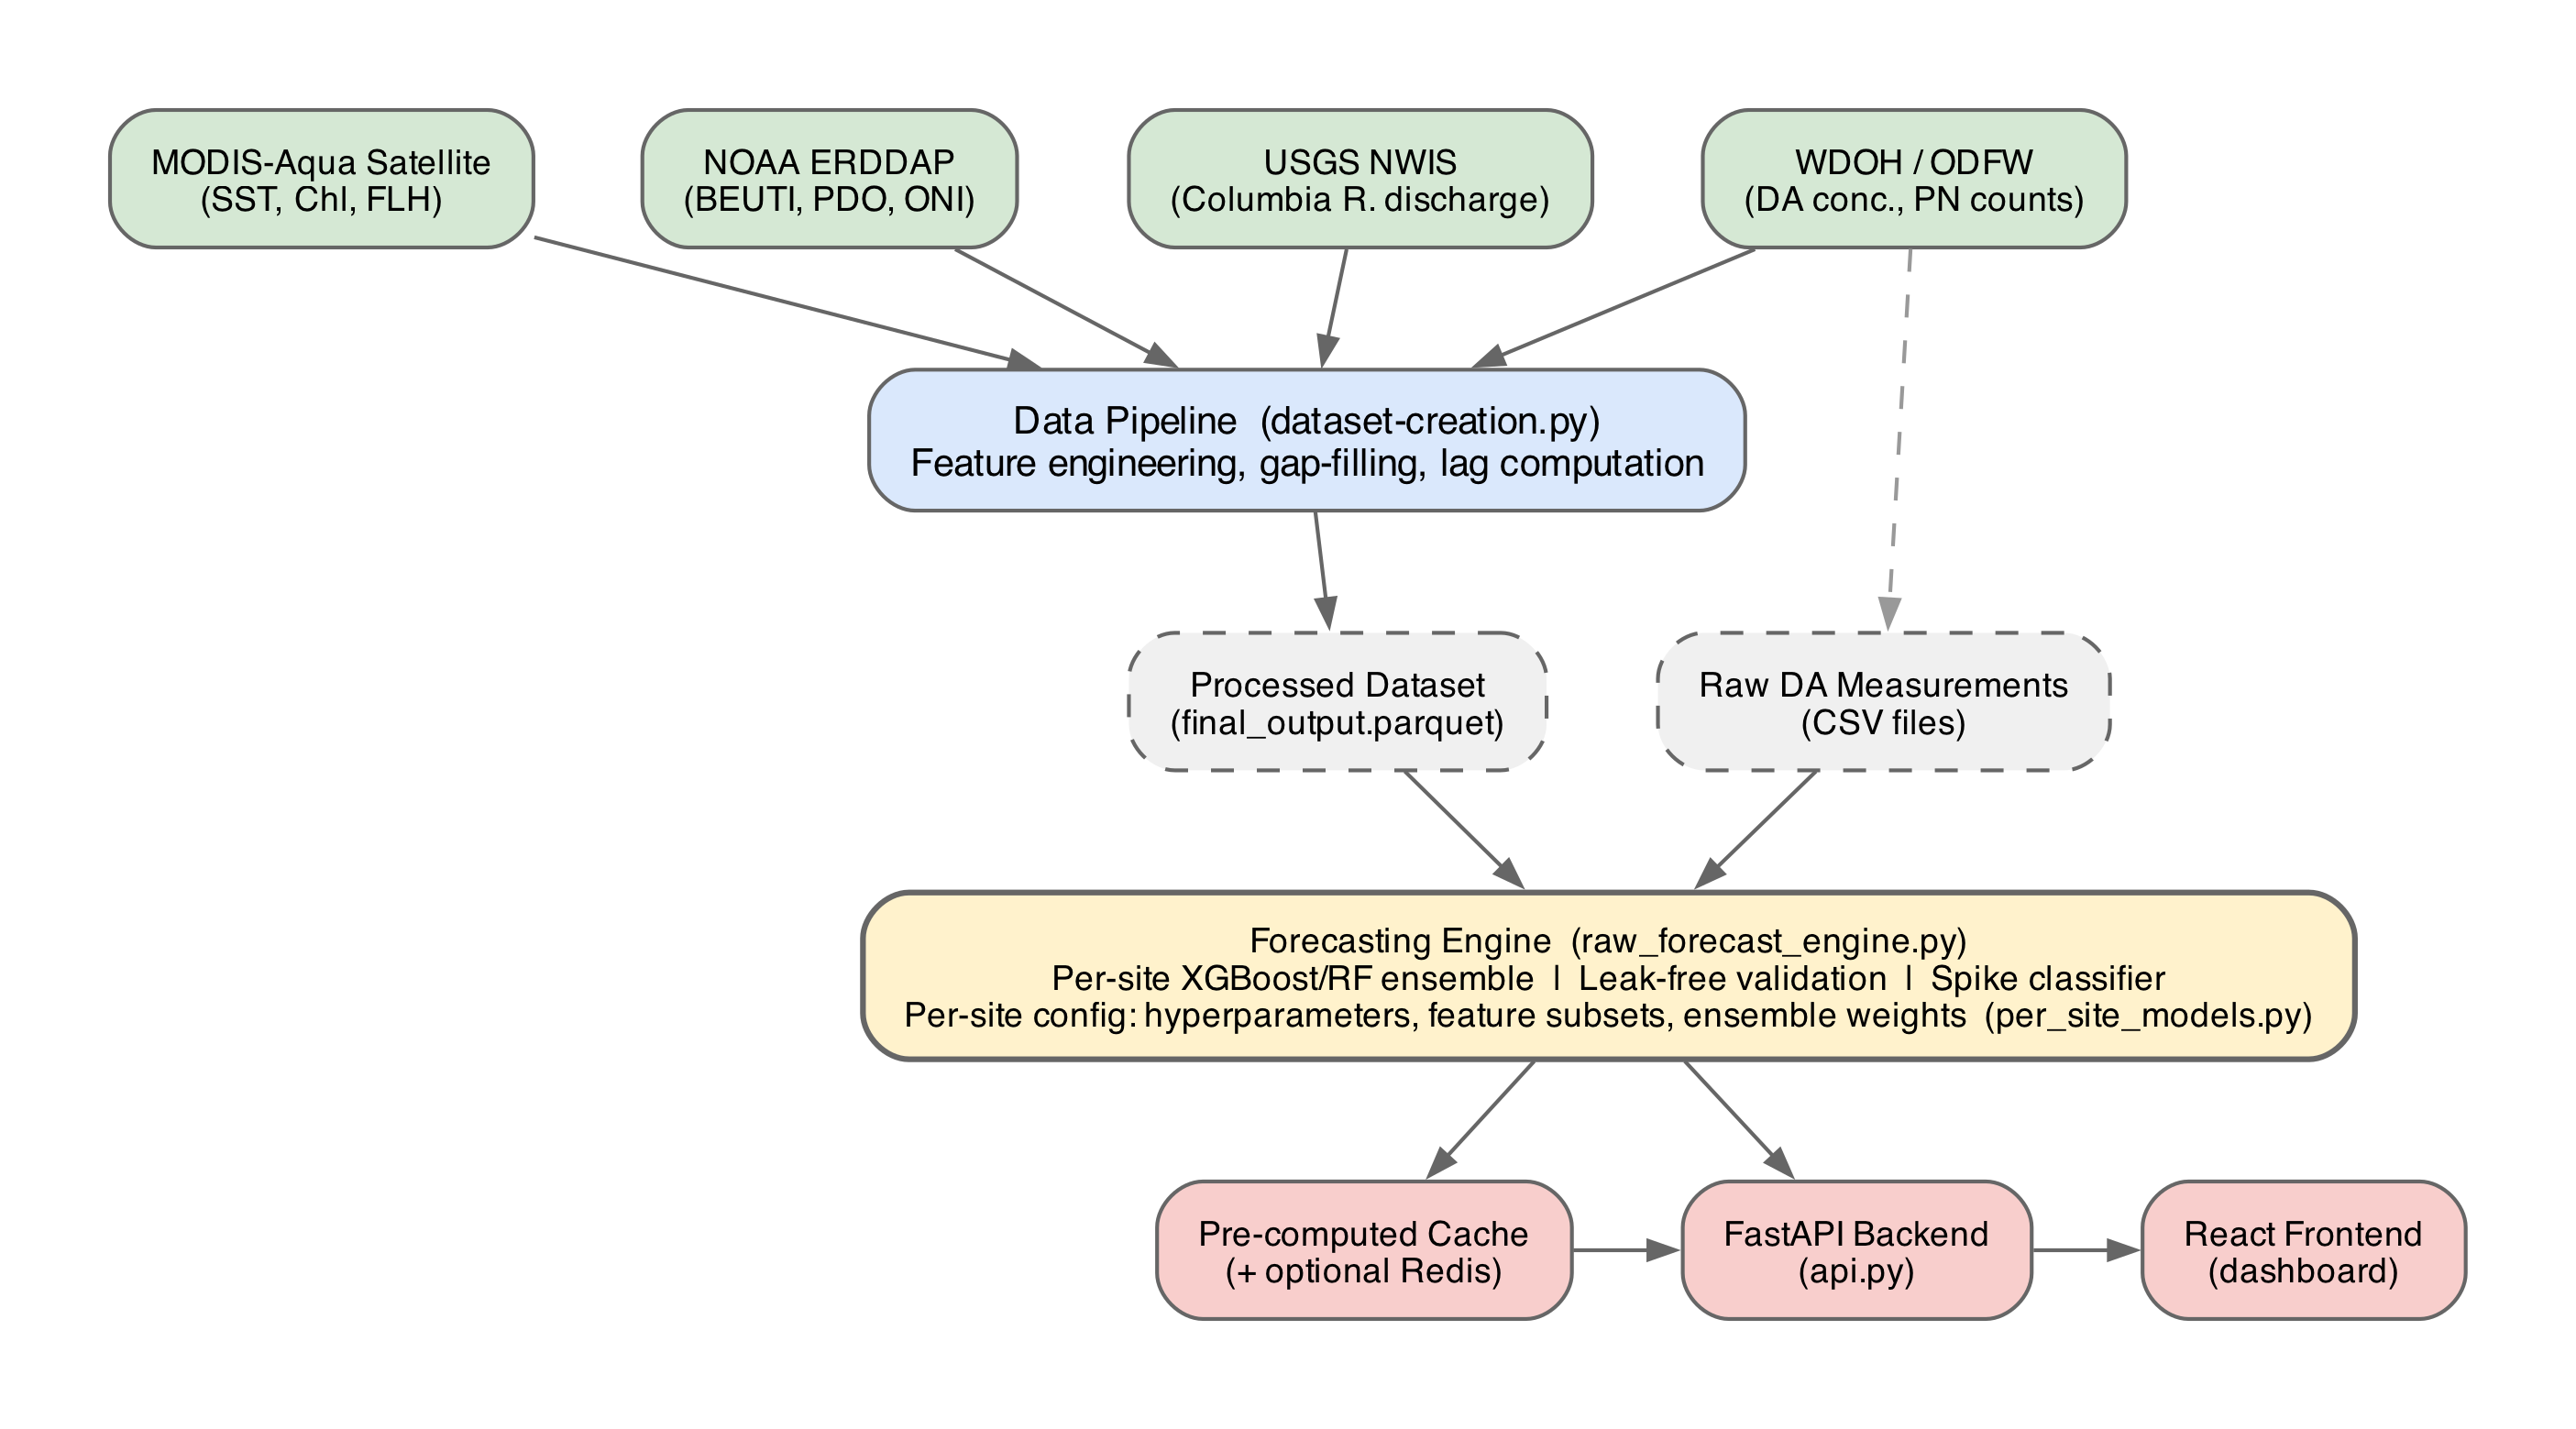
\includegraphics[width=\textwidth]{figures/fig3_architecture.png}
\caption{DATect system architecture: satellite, climate, hydrological, and biological data are processed into a unified dataset and served through a FastAPI backend to a React dashboard, with a pre-computed cache accelerating retrospective evaluations.}
\label{fig:architecture}
\end{figure}

The DATect backend serves forecast requests, retrospective evaluation results, and visualization data (correlation heatmaps, sensitivity analyses, spectral analyses, feature importance rankings). A pre-computed cache system stores results from computationally intensive retrospective evaluations as JSON and Parquet files, with an optional Redis backend providing 100$\times$ faster cache reads for production deployments. The retrospective evaluation cache---1,054 test points across 10 sites (the seed-42, 20\% development sample) for 8 model configurations---was pre-computed on the University of Washington Hyak high-performance computing cluster (\textit{klone} partition, STF allocation). Because each test point requires training a fresh ensemble on its own chronological training subset, the per-anchor computation is embarrassingly parallel and well-suited to HPC execution; running the full retrospective evaluation sequentially on a laptop would require several days, whereas the Hyak cluster completes the computation in approximately 2--3 hours across parallel jobs.

The system is containerized with Docker and deployed on Google Cloud Run, a serverless platform that scales to zero when idle and scales up to three concurrent instances under load. Cold start time is approximately 10--15 seconds. The deployment pipeline uses Google Cloud Build for continuous integration.

\subsection*{Operational Modes}

The dashboard supports two modes. In \textbf{real-time forecasting mode}, users select a target date and monitoring site; DATect trains a fresh model on all data up to the anchor date, returning a point prediction, 90\% confidence interval, risk category, and per-category probability distribution. In \textbf{retrospective analysis mode}, users select a model type and task to browse pre-computed validation results across all 1,054 cached test points, with interactive Plotly charts for scatter plots, confusion matrices, residual distributions, and time series overlays, filterable by site, date range, and DA risk category. Seven additional visualization types---including correlation heatmaps, sensitivity analyses, spectral density plots, SHAP-style feature waterfalls, and an interactive geographic map---are available for exploratory analysis. The live interface is available at the repository URL listed in the Data Availability Statement.


\section{Individual Feature Ablation}
\label{app:feature-ablation}

Table~\ref{tab:feature-ablation} presents a feature-group ablation of the final pipeline: each row removes one group of features that the models still use. No group changes $R^2$ by more than 0.004, and removing every environmental predictor at once costs only $\Delta R^2 = $-$0.004$: on this sample, regression skill comes almost entirely from the DA-history features. Features explored and removed during development are documented in Appendix~\ref{app:feature-engineering}.

\begin{table}[H]
\caption{Feature group ablation: each row removes one feature group from the full system, evaluated on the development sample (seed = 42, 20\%, $n = 1{,}054$).}
\label{tab:feature-ablation}
\centering\footnotesize
\begin{tabularx}{\linewidth}{Xcccc}
\toprule
\textbf{Feature(s) removed} & $\boldsymbol{R^2}$ & $\boldsymbol{\Delta R^2}$ & \textbf{MAE} & $\boldsymbol{\Delta}$\textbf{MAE} \\
\midrule
Full DATect (baseline) & 0.332 & --- & 6.29 & --- \\
\addlinespace
Satellite (SST, SST anomaly, FLH) & 0.335 & +0.003 & 6.28 & $-$0.01 \\
Climate indices (PDO, ONI) & 0.333 & +0.001 & 6.30 & +0.01 \\
Upwelling (BEUTI) & 0.332 & $-$0.000 & 6.29 & +0.01 \\
River discharge & 0.332 & $-$0.000 & 6.29 & +0.00 \\
\textit{Pseudo-nitzschia} (count, log count) & 0.332 & +0.000 & 6.29 & $-$0.00 \\
Rolling DA statistics (7) & 0.331 & $-$0.001 & 6.30 & +0.01 \\
Calendar (month, day-of-year sin/cos) & 0.334 & +0.002 & 6.30 & +0.01 \\
\addlinespace
All environmental (9)$^\dagger$ & 0.328 & $-$0.004 & 6.29 & +0.01 \\
\bottomrule
\end{tabularx}
\vspace{0.3em}\\
\footnotesize{Each group is dropped from every site's feature set; sites whose feature subset already excludes a group are unaffected. $\Delta$ values are paired on identical test points. $^\dagger$Satellite, climate indices, BEUTI, river discharge and \textit{Pseudo-nitzschia}.}
\end{table}


\section{Feature Importance Analysis}
\label{app:feature-importance}

\begin{figure}[H]
\centering
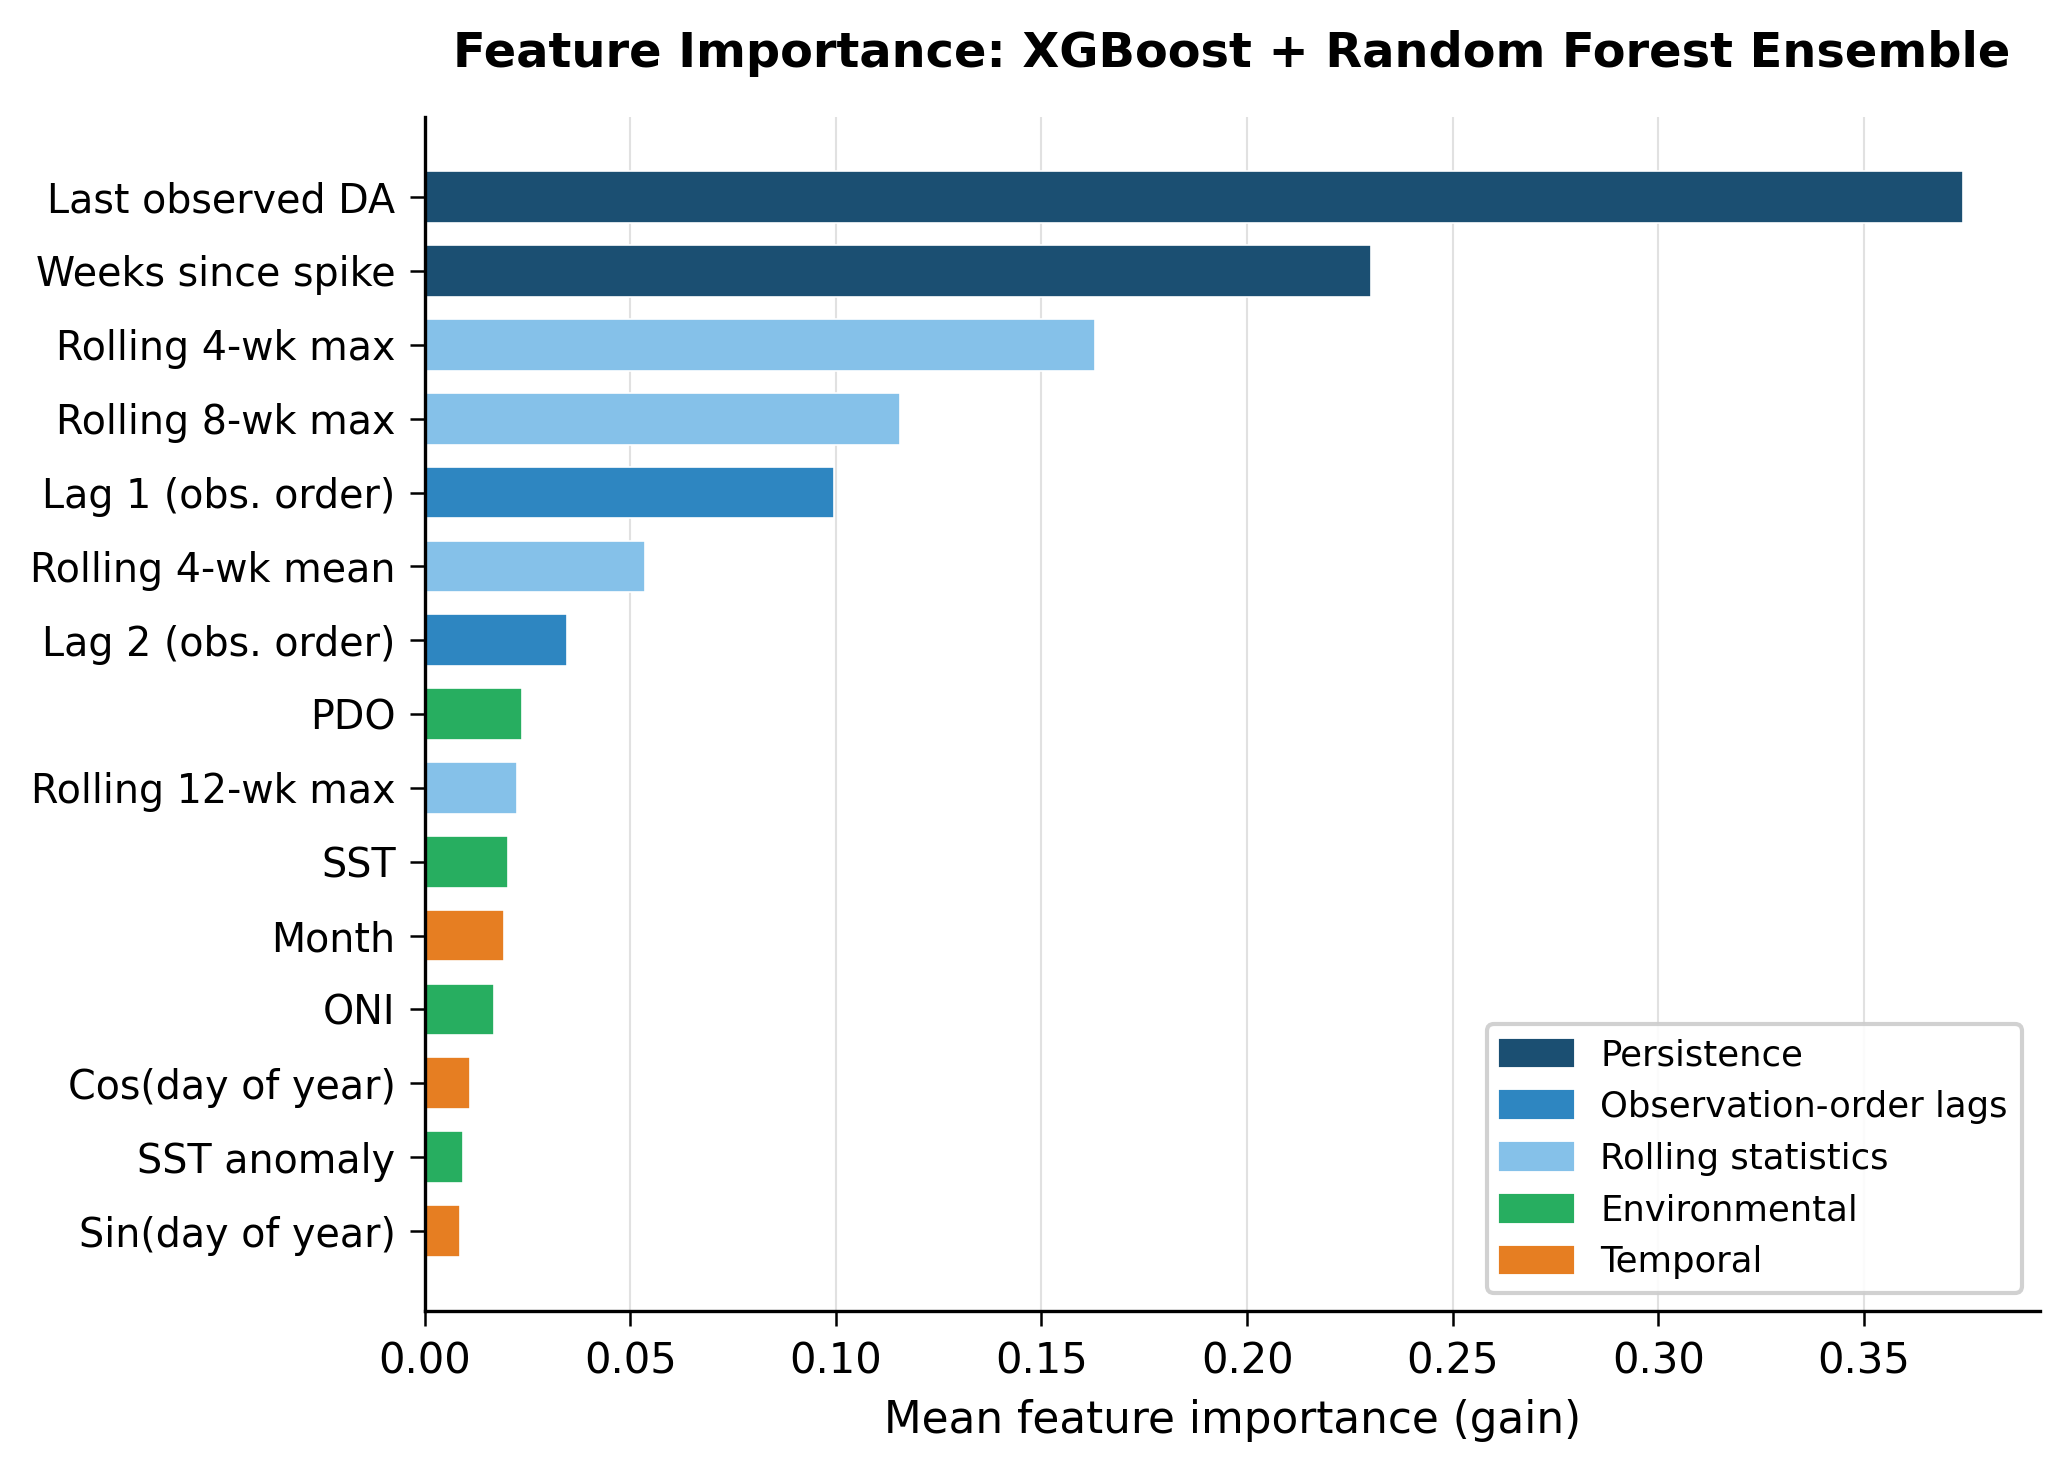
\includegraphics[width=0.85\textwidth]{figures/fig6_feature_importance.png}
\caption{Mean feature importance (gain) across all development-set predictions ($n = 1{,}054$), averaged over per-site ensemble models and color-coded by category (see Section~\ref{sec:results-ablation} for interpretation).}
\label{fig:feature-importance}
\end{figure}


\section{Model Selection Robustness}
\label{app:weight-robustness}

Since DATect assigns each site a single model (XGBoost or Random Forest) based on development-set performance, weight robustness reduces to model-selection robustness: how sensitive are aggregate results to the per-site XGB vs.\ RF choice? Table~\ref{tab:weight-robustness} compares four strategies evaluated on the held-out test set ($n = 2{,}105$, seed = 123).

\begin{table}[H]
\caption{Model-selection robustness on the held-out test set ($n = 2{,}105$, seed = 123).}
\label{tab:weight-robustness}
\centering\small
\begin{tabular*}{\linewidth}{@{\extracolsep{\fill}}lccc}
\toprule
\textbf{Strategy} & \textbf{$R^2$} & \textbf{MAE (\si{\microgrampeg})} & \textbf{RMSE (\si{\microgrampeg})} \\
\midrule
XGBoost at all sites                    & 0.331 & 6.78 & 19.51 \\
RF at all sites                         & 0.330 & 6.42 & 19.52 \\
Per-site dev-set selection (this paper) & 0.337 & 6.53 & 19.42 \\
Linear/Ridge at all sites               & 0.325 & 6.61 & 19.59 \\
\bottomrule
\end{tabular*}
\end{table}

The near-equivalence of these strategies ($R^2 = 0.325$--$0.337$, all within their pairwise bootstrap CIs; Table~\ref{tab:model-comparison}) confirms that model-family selection is not a meaningful source of variance. Per-site dev-set selection (the ensemble formulation used throughout this paper) has the highest point estimate, ahead of XGBoost-everywhere (0.331) and RF-everywhere (0.330), but the differences are well within the 5-seed bootstrap dispersion ($\sigma \approx 0.05$ at this $N$; see Section~\ref{sec:results-temporal-holdout}). The ensemble formulation is retained for generality and because per-site selection enables site-specific feature subsets and clipping (Appendix~\ref{app:hyperparams}).


\section{Perturbation Sensitivity Analysis}
\label{app:perturbation-sensitivity}

To test whether per-site design choices are fragile, we run a systematic perturbation study. Each experiment modifies a single design dimension while holding all others fixed, evaluated on the development sample ($n = 1{,}054$, seed = 42, 20\% sample). Table~\ref{tab:perturbation} reports the results.

\begin{table}[H]
\caption{Perturbation sensitivity analysis: each row modifies one design choice relative to the baseline ($R^2 = 0.332$), evaluated on the development sample (seed = 42, $n = 1{,}054$).}
\label{tab:perturbation}
\centering\footnotesize
\begin{tabularx}{\linewidth}{Xrrr}
\toprule
\textbf{Perturbation} & $\boldsymbol{R^2}$ & $\boldsymbol{\Delta R^2}$ & \textbf{MAE} \\
\midrule
\multicolumn{4}{l}{\textit{Model selection}} \\
\quad XGBoost at every site & 0.331 & $-$0.001 & 6.40 \\
\quad RF at every site & 0.323 & $-$0.009 & 6.23 \\
\quad No per-site config & 0.327 & $-$0.005 & 6.14 \\
\midrule
\multicolumn{4}{l}{\textit{RF hyperparameters}} \\
\quad Shallow (dep.\ 6, $n_{\text{est}}$ 200) & 0.332 & +0.000 & 6.27 \\
\quad Deep (dep.\ 16, $n_{\text{est}}$ 600) & 0.332 & $-$0.000 & 6.29 \\
\quad More trees ($n_{\text{est}}$ 800) & 0.332 & +0.000 & 6.29 \\
\quad Less reg.\ (leaf = 1) & 0.332 & $-$0.000 & 6.29 \\
\midrule
\multicolumn{4}{l}{\textit{Feature \& clipping}} \\
\quad All features all sites & 0.347 & +0.015 & 6.25 \\
\quad Minimal features (4) & 0.333 & +0.001 & 6.49 \\
\quad Relax clip ($q = 0.99$) & 0.371 & +0.039 & 6.13 \\
\quad Disable clipping & 0.388 & +0.055 & 6.08 \\
\quad Disable monotonic & 0.332 & +0.000 & 6.29 \\
\bottomrule
\end{tabularx}
\vspace{0.3em}\\
\footnotesize{Rows are paired on identical test points. RF variants change the global RF parameters; the four sites with their own RF parameters (Coos Bay, Cannon Beach, Gold Beach, Newport) keep them. Every change is passed to the parallel training workers as an environment variable (\texttt{scripts/eval/paper\_sensitivity\_study.py}).}
\end{table}

Three findings emerge. First, Random Forest hyperparameters are insensitive: across four configurations spanning depth 6--16 and 200--800 trees, no perturbation exceeds $|\Delta R^2| = 0.001$, and removing the monotonic constraints changes nothing. Second, model-family and feature-subset choices matter little: XGBoost or Random Forest at every site, no per-site configuration, and a four-feature persistence-only subset all stay within 0.01 of the baseline, while using every feature at every site gains $+0.015$. Third, prediction clipping now costs skill: relaxing every per-site quantile to 0.99 gains $+0.039$ and removing clipping gains $+0.055$ (MAE 6.08 vs.\ 6.29). The per-site clip quantiles (0.95--0.97) were selected by the grid search before the evaluation targets were corrected to one measurement per site-day (Section~\ref{sec:retro-eval}); against daily-maximum targets, a cap at the 95th--97th percentile of training targets truncates real spikes. This sample includes 2022--2023 rows, so it cannot be used to choose new clip values; re-running the leak-free chronological grid search on the corrected targets is future work (Section~\ref{sec:discussion-limitations}).

Multi-seed evaluation further characterizes the stability of these results. Table~\ref{tab:seed-stability} reports per-site $R^2$ across the five bootstrap seeds (42--46) with per-site configuration enabled.

\begin{table}[H]
\caption{Per-site $R^2$ across the five bootstrap seeds (42--46; 20\% of all real DA measurements, $N = 1{,}054$ per seed; per-site configuration enabled). Sites are grouped by region.}
\label{tab:seed-stability}
\centering\scriptsize
\begin{tabular*}{\linewidth}{@{\extracolsep{\fill}}lrrrrrrr}
\toprule
\textbf{Site} & \textbf{s42} & \textbf{s43} & \textbf{s44} & \textbf{s45} & \textbf{s46} & \textbf{Mean} & \textbf{Std} \\
\midrule
\multicolumn{8}{l}{\textit{Washington}} \\
Copalis      & .825 & .779 & .797 & .719 & .792 & .783 & .039 \\
Kalaloch     & .559 & .703 & .471 & .598 & .576 & .581 & .084 \\
Twin Harb.   & .431 & .603 & .561 & .723 & .694 & .603 & .116 \\
Long Beach   & .303 & .554 & .532 & .499 & .637 & .505 & .124 \\
Quinault     & .527 & .426 & .494 & .233 & .367 & .409 & .117 \\
\midrule
\multicolumn{8}{l}{\textit{Oregon}} \\
Clatsop Bch  & .447 & .491 & .500 & .454 & .470 & .472 & .023 \\
Coos Bay     & .125 & .212 & .212 & .200 & .246 & .199 & .045 \\
Gold Beach   & .235 & $-$.119 & .263 & .186 & .070 & .127 & .156 \\
Cannon Bch   & $-$.048 & $-$.028 & $-$.018 & $-$.012 & $-$.039 & $-$.029 & .015 \\
Newport      & $-$.018 & $-$.208 & .139 & $-$.029 & $-$.139 & $-$.051 & .132 \\
\midrule
Pooled       & .332 & .392 & .395 & .292 & .314 & .345 & .046 \\
\bottomrule
\end{tabular*}
\end{table}

Washington sites are consistently skillful across seeds (mean $R^2 = 0.41$--$0.78$, std 0.04--0.12), and Clatsop Beach is the most stable site of all ($0.47 \pm 0.02$). The four other Oregon sites stay near zero in every seed (means $-0.05$ to $0.20$, std up to 0.16 at Gold Beach). The skill divide persists across all five seeds, so it reflects the sites' data and DA dynamics rather than seed-specific sampling.


% ══════════════════════════════════════════════════════════════════════════════
%  REFERENCES
% ══════════════════════════════════════════════════════════════════════════════
\externalbibliography{yes}
\bibliography{references}

\end{document}
